\section{Experimental Evaluation}
\label{sec:experiments}

This this section we present a detailed experimental evaluation of \VizRecDB.
With the use of real and synthetic datasets, we performed an extensive
investigation of both execution engines of \VizRecDB. 
Our goals were to study the performance characteristics of \VizRecDB along with
the correctness and accuracy of our heuristics.
All experiments were run on a
single machine with 8 GB RAM and a 16 core Intel Xeon E5530 processor .

We begin with an evaluation of the DBMS-backed execution engine followed by an
evaluation of our custom solution.

\subsection{DBMS-backed Execution Engine}
\label{sec:expts_dbms_execution_engine}

As mentioned in Section \ref{sec:dbms_execution_engine}, our DBMS-based
execution engine leverages the DBMS API to execute view queries directly on the
database.
While this approach has the advantages of reusing existing query procesing
systems and being agnostic to the specific underlying DBMS, its limitations
include the lack of fine grained control over sharing of table scans and lack of
ability to prune low-utility views. 
In this set of experiments, we investigate how well existing DBMSs can support a
\VizRecDB\ style workload in the presence of the right optimizations.
The metric we are concerned is latency -- what was the total time taken by
\VizRecDB\ to compute the top views for any given query.
All latency measurements were repeated three times and the results were
averaged.
Since this version of the execution engine exhaustively explores all views and
then orders them by utility, we are guaranteed to get the top-$k$ views with
perfect accuracy.

We ran all our experiments in this section on two database systems: a
row-oriented database (denoted as ROW in the following figures) and a
column-oriented database (COL).
The reason for evaluating both systems was that we expect (and
demonstrate below) that certain optimizations to work better for row-stores vs.
column stores.
We start with an evaluation of the basic framework and then study the effect of
adding each individual optimization.\\

\noindent {\it Basic Framework}: The basic DBMS-backed execution engine
sequentially executes individual view queries for each possible view.
Figure \ref{fig:baseline_size} and Figure \ref{fig:baseline_views} show the
\VizRecDB\ latency when using the basic framework.
Figure \ref{fig:baseline_size} shows the change in latency with changes in table
size while Figure \ref{fig:baseline_views} shows the impact of view number on
the latency.
In Figure \ref{fig:baseline_size}, we fixed the number of views at 250 and
varied the number of rows from 100K to 1M, whereas in Figure
\ref{fig:baseline_views}, we fixed the number of rows at 1M and varied the
number of views from 50 - 250.
As expected, we see that the latency of the basic framework is directly
proportional to the number of rows as well as the number of views in the table.
We see that the column store runs wildly faster than the row store in each run.
This is expected because individual view queries only select one dimension
attribute and one measure attribute at a time, making each query in the column
store significantly faster than the same query in the row store which must load
all columns.

Finally, we note that the row and column store respectively take between 10-100s
and between 50-500s to evaluate all views.
These time scales are simply unacceptable for interactive applications, and
therefore, we must aggressively optimize our queries. \\

% \begin{figure}[h] 
% \centerline{
% \resizebox{4cm}{!} {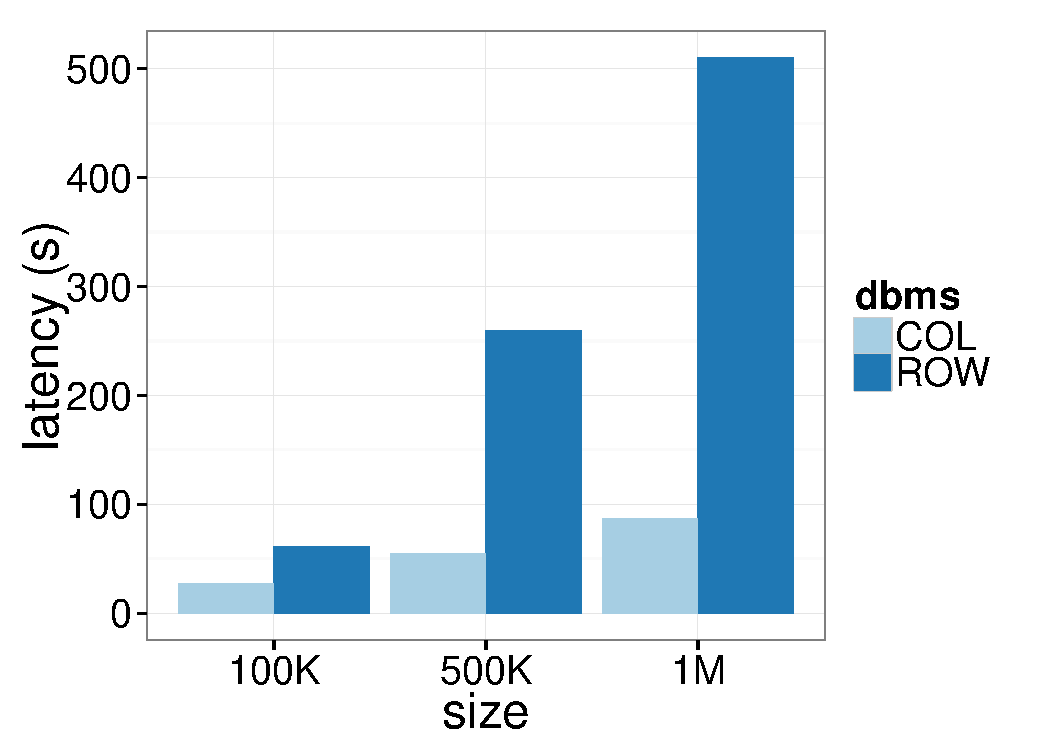
\includegraphics {Images/baselines_by_size.pdf}}
% \resizebox{4cm}{!} {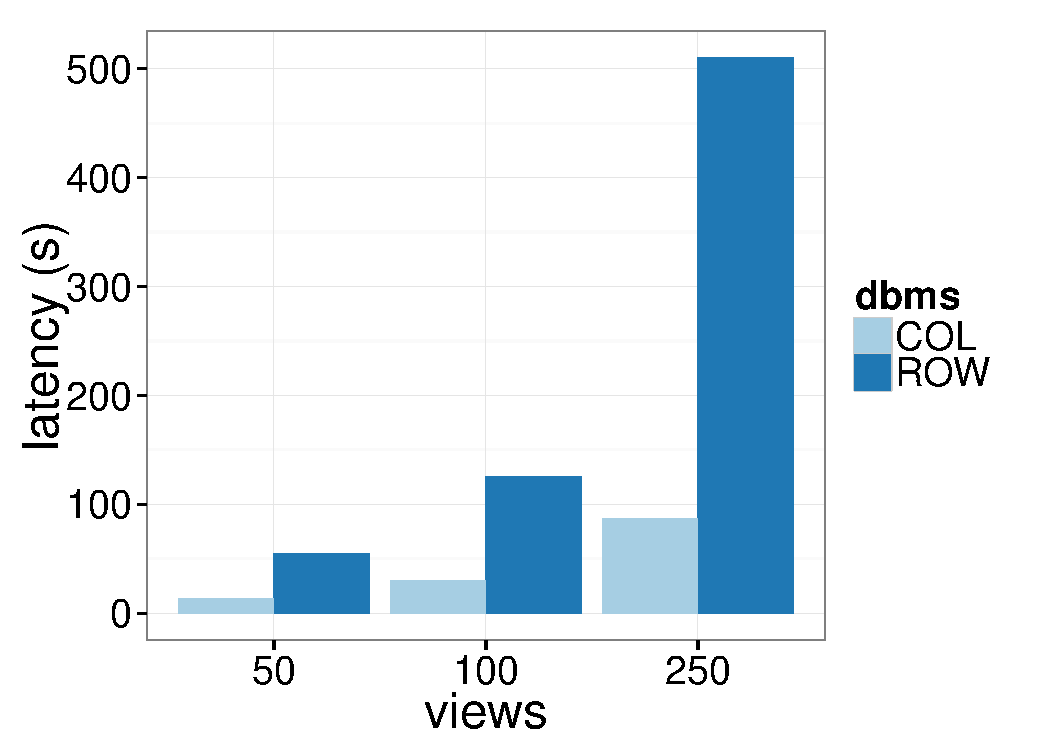
\includegraphics {Images/baselines_by_views.pdf}}
% }
% \end{figure}

\begin{figure*}[t]
	\centering
	\begin{subfigure}{0.33\linewidth}
		{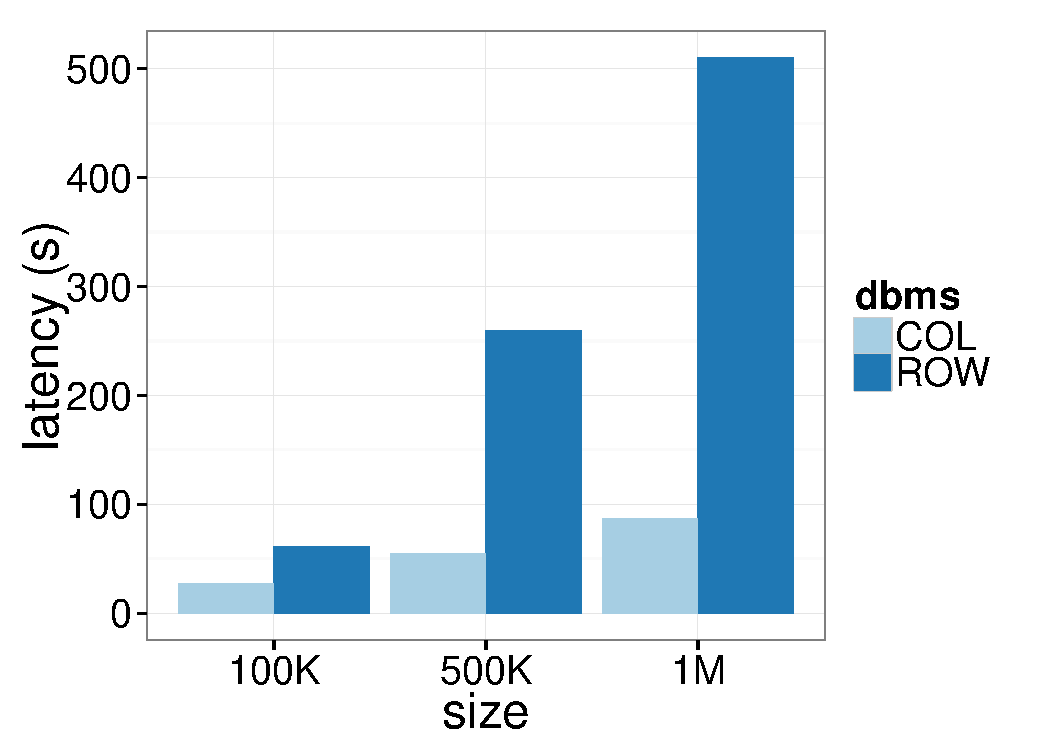
\includegraphics[width=6cm] {Images/baselines_by_size.pdf}}
		\caption{Latency vs. Table size}
		\label{fig:baseline_size}
	\end{subfigure}
	\begin{subfigure}{0.33\linewidth}
		\centering
		{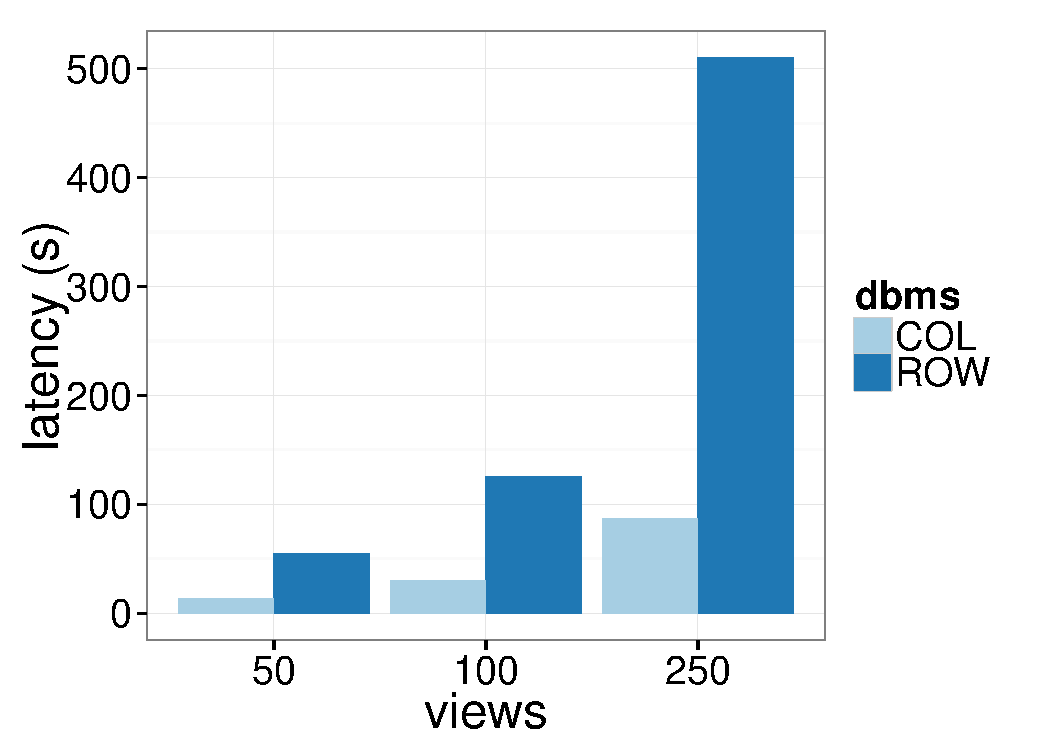
\includegraphics[width=6cm] {Images/baselines_by_views.pdf}}
		\caption{Latency vs. Num Views}
		\label{fig:baseline_views}
	\end{subfigure}
	\begin{subfigure}{0.33\linewidth}
		\centering
		{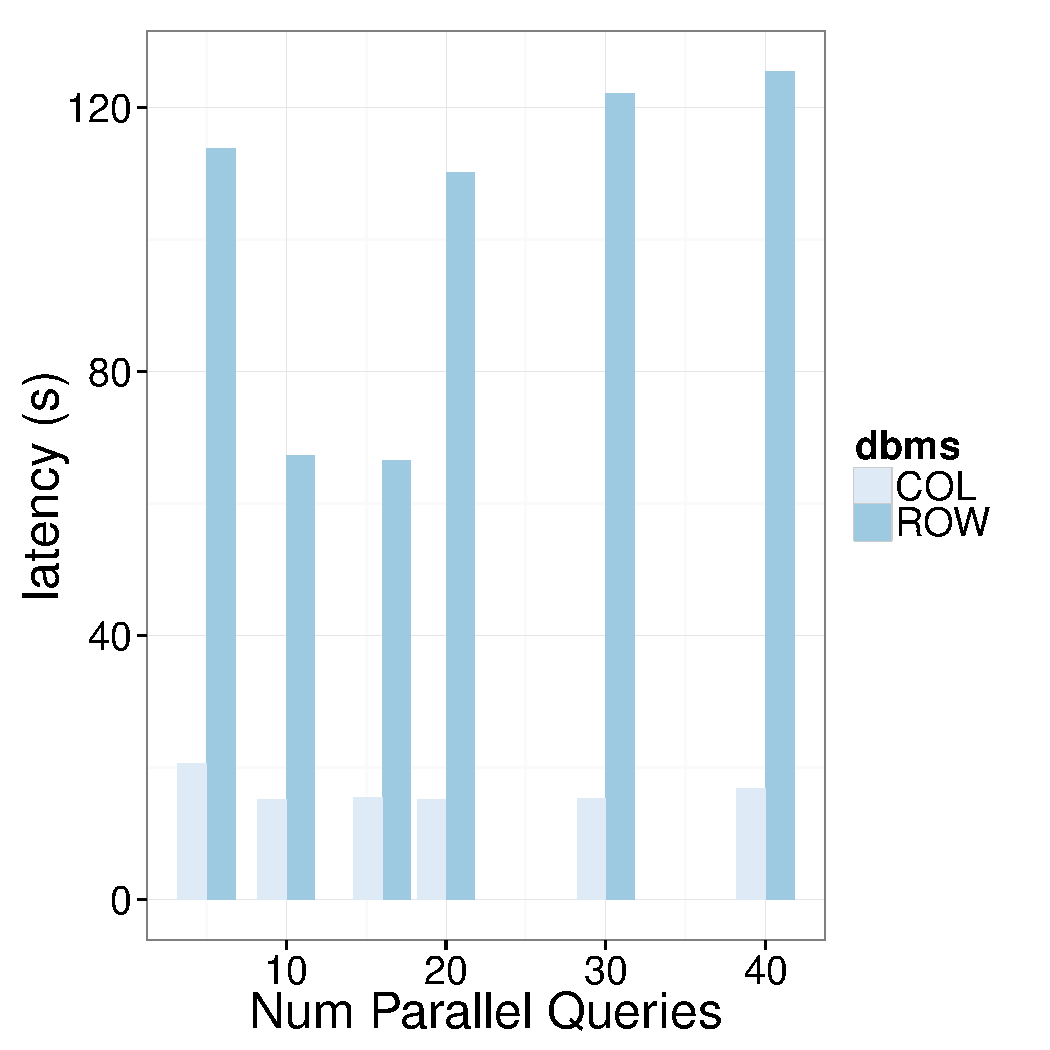
\includegraphics[width=6cm] {Images/parallel_noop.pdf}}
		\caption{Effect of parallelism}
		\label{fig:parallelism}
	\end{subfigure}
	\caption{Baseline performance and Effect of Parallel Query Execution}
	\label{fig:bank_perf}
\end{figure*}

\begin{figure*}[t]
	\centering
	\begin{subfigure}{0.33\linewidth}
		{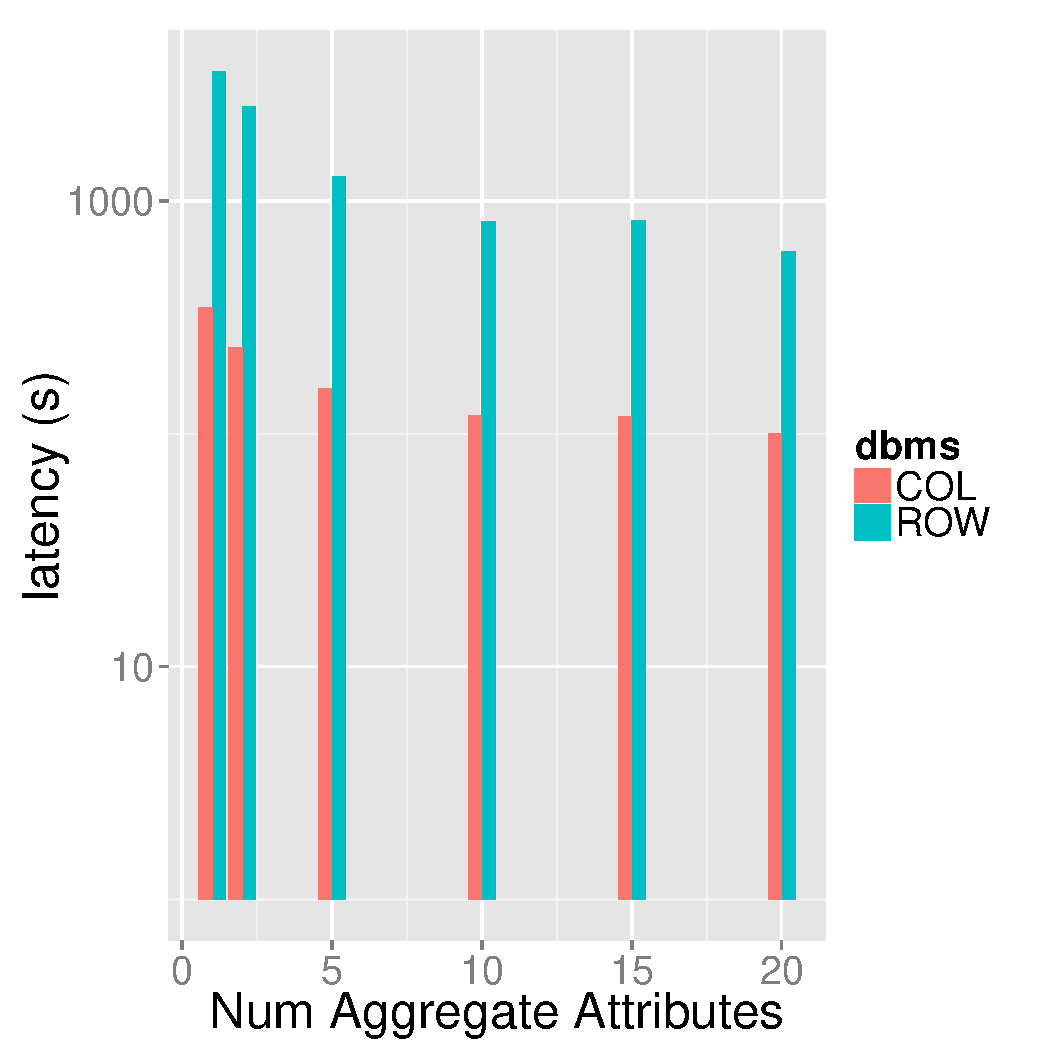
\includegraphics[width=6cm] {Images/multi_agg.pdf}}
		\caption{Latency vs. number of aggregates}
		\label{fig:multi_agg}
	\end{subfigure}
	\begin{subfigure}{0.33\linewidth}
		\centering
		{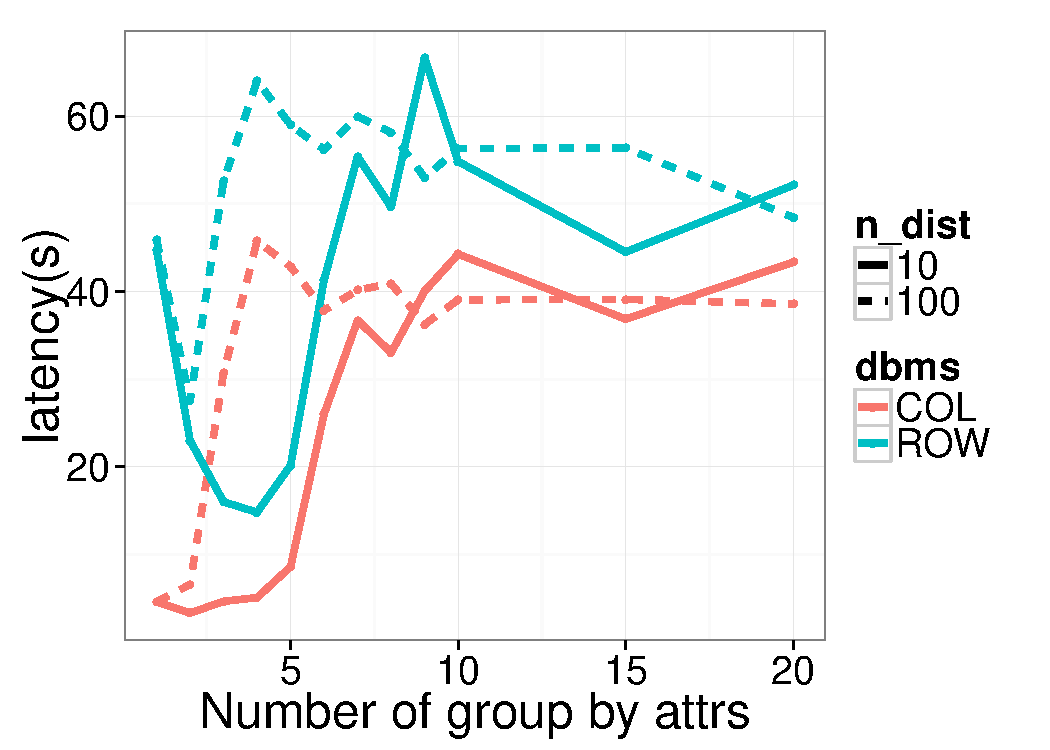
\includegraphics[width=6cm] {Images/multi_gb_same.pdf}}
		\caption{Latency vs. Num of Groups}
		\label{fig:multi_gb_same}
	\end{subfigure}
	\begin{subfigure}{0.33\linewidth}
		\centering
		{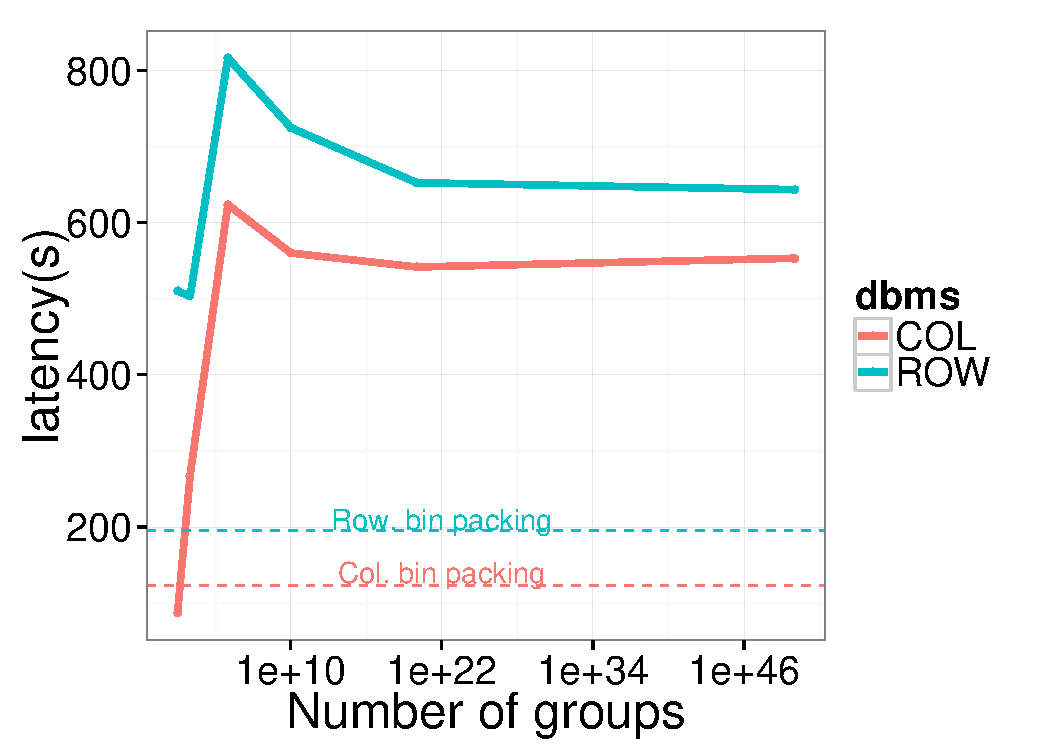
\includegraphics[width=6cm] {Images/multi_gb.pdf}}
		\caption{Latency vs. Num Dimensions}
		\label{fig:multi_gb_bp}
	\end{subfigure}
	\caption{Effect of Combining Multiple Queries}
	\label{fig:bank_perf}
\end{figure*}

% \begin{figure}[h]
% \centering
% \begin{subfigure}{0.49\linewidth}
% \centering
% {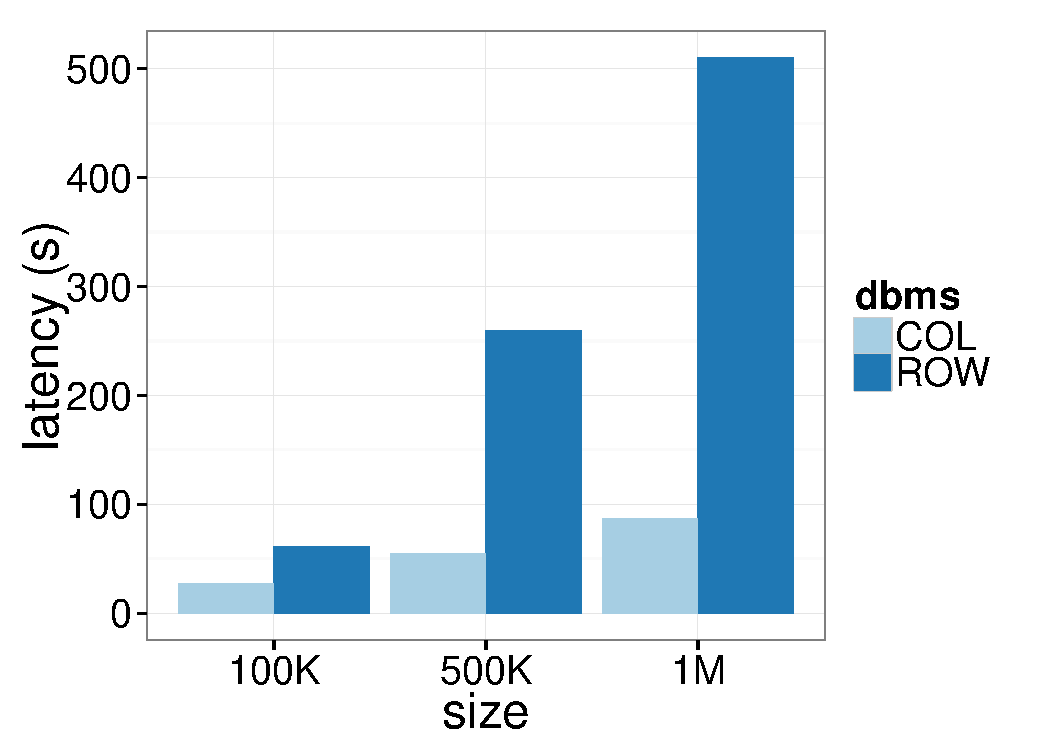
\includegraphics[width=4.2cm] {Images/baselines_by_size.pdf}}
% \caption{Latency vs. Table size}
% \label{fig:baseline_size}
% \end{subfigure}
% \begin{subfigure}{0.49\linewidth}
% \centering
% {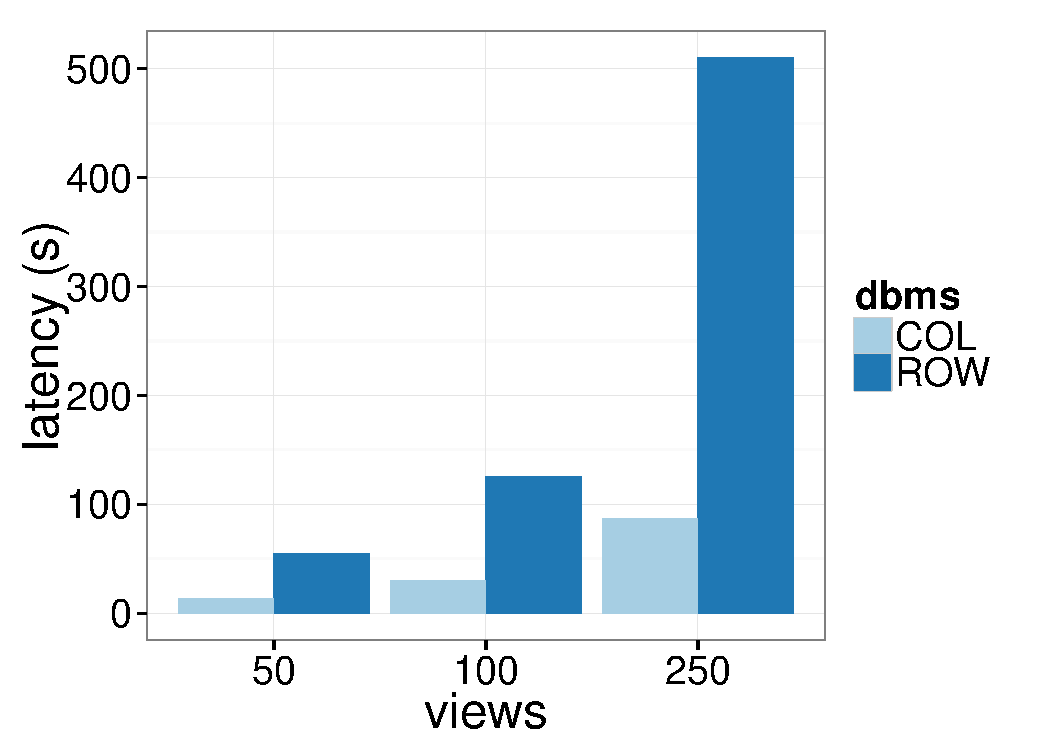
\includegraphics[width=4.2cm] {Images/baselines_by_views.pdf}}
% \caption{Latency vs. Num Views}
% \label{fig:baseline_views}
% \end{subfigure}
% \label{fig:baselines}
% \caption{Latency of Basic Framework}
% \end{figure}

\noindent {\it Combining Multiple Aggregates}: Next, we study the impact of
combining multiple aggregates within the same query.
The goal of this optimization is to evaluate multiple views at once by keeping
track of multiple aggregates for the same dimension attribute.
For a synthetic dataset of 1M rows and 1000 views (50 dimension and 20 measure
attributes), we varied the number of aggregations performed per query
($n_{agg}$) between 1 and 20 and measured the impact on latency.
As shown in Figure \ref{fig:multi_agg}, latency reduces as we increase the
number of aggregations performed per query.
This optimization shows promise both in the row store as well as the column
store, athough we note that the optimization has diminishing returns because it
requires more state to be stored and, in the case of the column stores, more
columns to be read. \\

% \begin{figure}[h]
% \centering
% {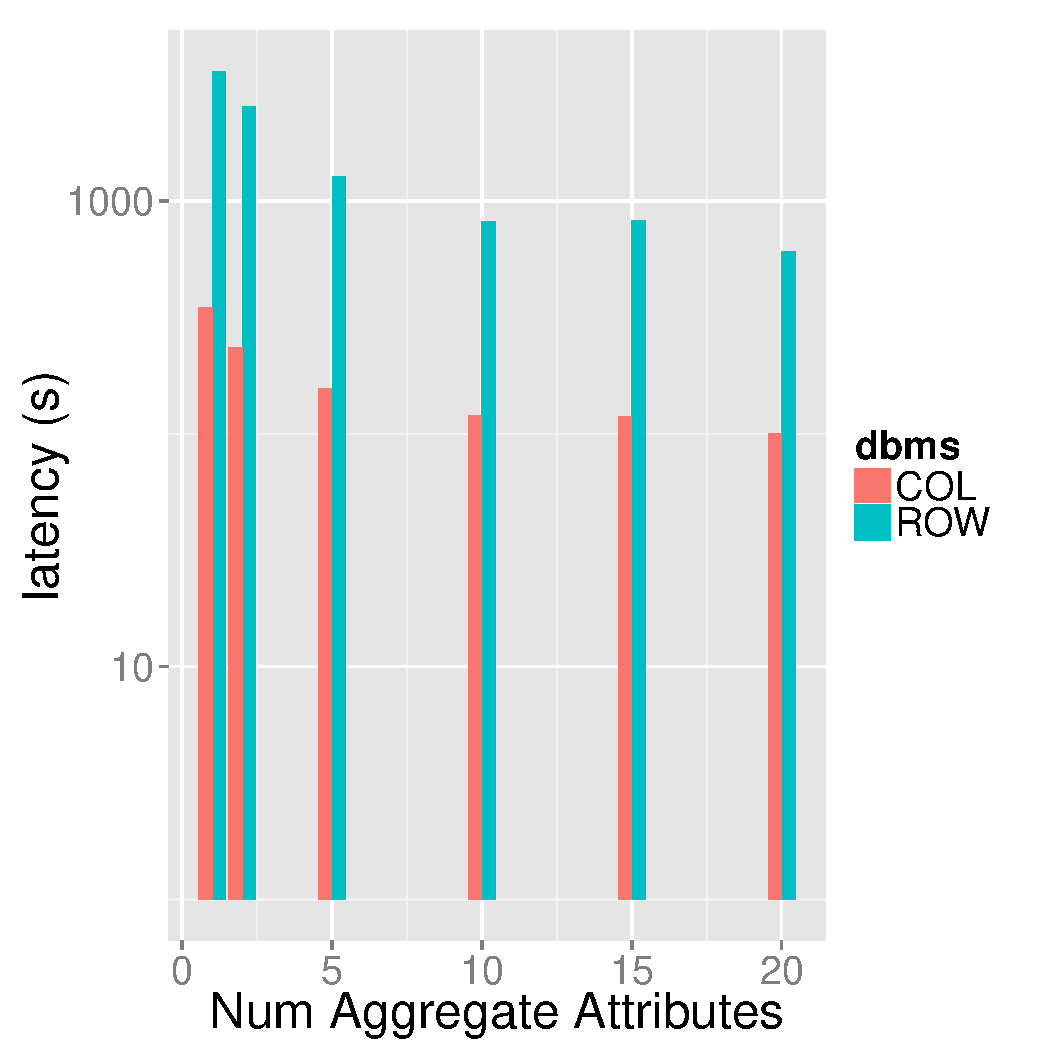
\includegraphics[width=6cm] {Images/multi_agg.pdf}}
% \caption{Latency vs. number of aggregates}
% \label{fig:multi_agg}
% \end{figure} 

\noindent {\it Combining Multiple Group Bys}: In this set of experiments, we
study the effect of combining multiple group by attributes into one query.
Section \ref{} briefly discussed how the impact of this optimization was not
clear since it increases the total number of groups significantly and therefore
leads to higher cost of processing intermediate results.
To evaluate this optimization, we generated a synthetic dataset with 1M rows, 1
measure attribute and 20 dimension attributes such that each dimension attribute
was independently generated and had exactly 10 distinct values.
Since each dimension attribute is independent of the others and has 10 distinct
values, the total number of distinct groups produced by a query
with $p$ group-by attributes is $10^p$.

We ran \VizRecDB\ on this dataset and varied the number of group-by
attributes in view queries ($n_{gb}$) between 1 and 20.
Figure \ref{fig:multi_gb_same} shows the results for this experiment.
We see that for the row-store, the best latency is obtained for number of
groups=$10^4$.
Beyond $10^5$, the performance degrades drastically. 
For the column-store, we see a relatively small improvement in latency
for $10^2$ groups, however, once again, after $10^5$ groups, the performance
becomes much worse.
The reason for this is as follows: as we combine group by attributes, the number
of distinct groups increases exponentially ($10^{n_{gb}}$). 
As a result, the memory required for the grouping (hash-based or sort based)
also increases significantly.
Once this memory requirement hits the pre-configured upper limit (e.g. say the
memorycap in the column store or working memory in the row store), the
performance degrades significantly.

% \begin{figure}[h]
% \centering
% \begin{subfigure}{0.49\linewidth}
% \centering
% {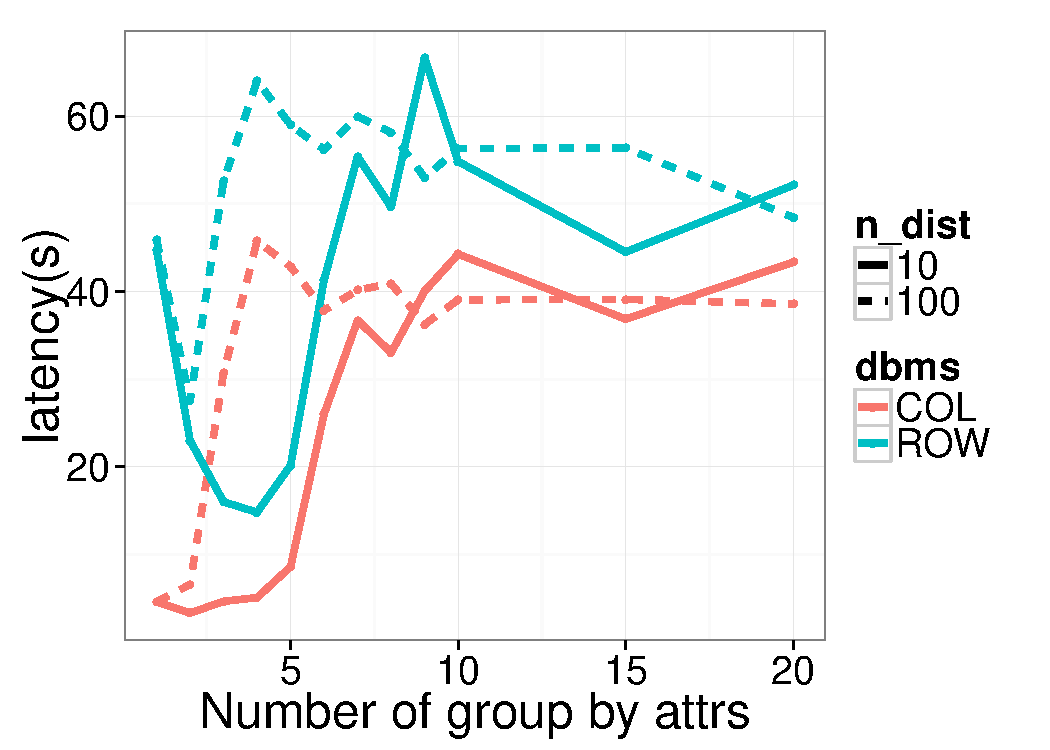
\includegraphics[width=4.2cm] {Images/multi_gb_same.pdf}}
% \caption{Latency vs. Num of Groups}
% \label{fig:multi_gb_same}
% \end{subfigure}
% \begin{subfigure}{0.49\linewidth}
% \centering
% {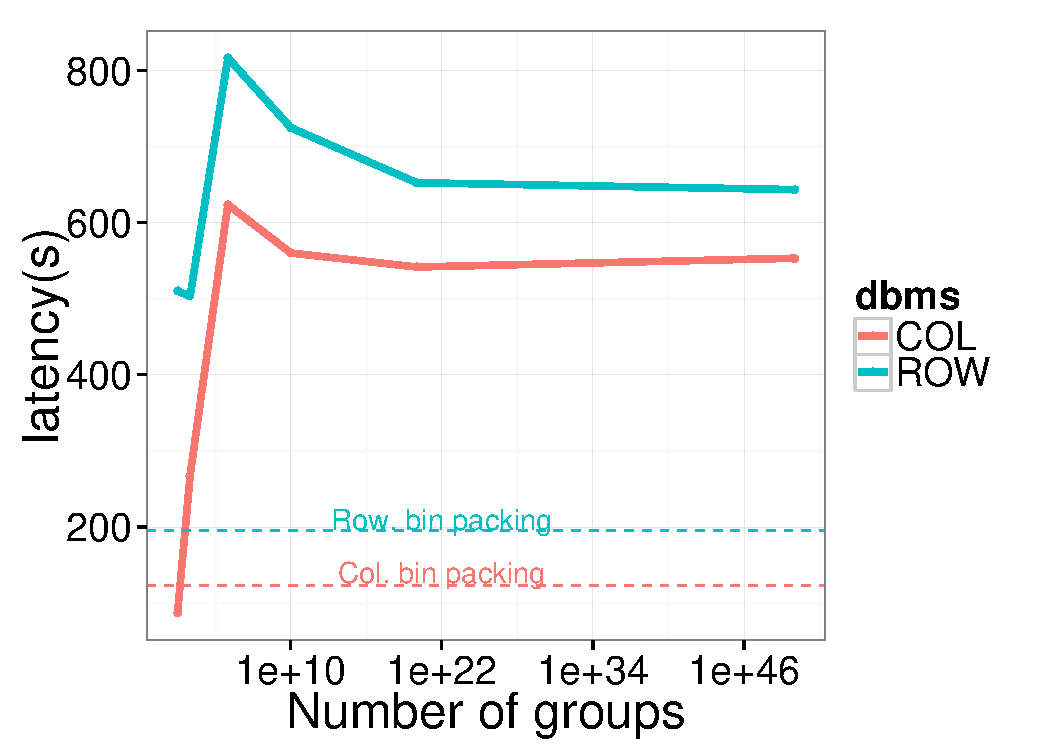
\includegraphics[width=4.2cm] {Images/multi_gb.pdf}}
% \caption{Latency vs. Num Dimensions}
% \label{fig:multi_gb_bp}
% \end{subfigure}
% \label{fig:multi_gb}
% \caption{Effect of combining multiple groups}
% \end{figure}

We can guard against the above performance degradation by ensuring that the
number of distinct groups never goes beyond a pre-configured upper limit.
From Figure \ref{fig:multi_gb_same}, we see that this limit is approximately
$10^5$ for both the row and column store.
With knowledge of this upperlimit on the number of distinct groups, we can
now apply the bin packing technique discussed in Section \ref{} to optimally
group the attributes. 
Bin-packing ensures that the number of distinct groups produced by any
query is less than $10^5$. 
Figure \ref{fig:multi_gb_bp} shows the results of combining group-by attributes
for a synthetic dataset with  1M rows, 50 dimension, 5 measures and with varying
number of distinct values in each dimension attribute. 
% There are two opposing forces at work here: increasing the number of dimensions
% in a query increases the execution time for that query, however, it reduces the
% number of queries that must be executed and hence reduces execution time.
We see trends similar to those in Figure \ref{fig:multi_gb_same} (notice that
\ref{fig:multi_gb_same} has a log scale on the x-axis).
The horizontal lines denote the performance of the bin-packing heuristic that
optimally groups dimension attributes keep the number of groups below the
upper limit.
We see that for the row-store, bin-packing halves even the best latency for
other group-by combinations. 
The column store on the other hand doesn't appear to benefit from this
optimization. 
Bin-packing gives approximately the same (in fact slightly worse) performance as
not combining group-bys attributes. \\

\noindent {\it Parallel Query Execution}: 
Executing view queries in parallel can provide significant performance gains;
however, a high degree of parallelism can lead to a performance drop off for
several reasons. Potential reasons include disk contention, RAM usage, lock
contention, context switches and cache line contention \cite{Postgres_wiki}. 
Figure \ref{fig:parallelism} illustrates this issue: we varied the number of
queries running in parallel on the DBMS and measured the latency of
\VizRecDB.
As expected, low levels of parallelism produce sizable performance gains but
high parallelism leads to degraded performance.
For our system, the optimal number of queries to run in parallel is
approximately $16$ (equal to the number of cores).
For other systems, we recommend users that they set the number of parallel
queries to the maximum number of parallel queries that can be run in
their DBMS without performance degradation.
If this number is not easily available, a simple experiment as shown in Figure
\ref{fig:parallelism} can help approximate the right amount of parallelism. \\

\noindent {\it Combining Target and Comparison Views}:
The last optimization we evaluate is that of combining the target and comparison
views and running a single SQL query per view as opposed to two.
We expected this optimization to roughly halve the latency since each query
takes one table scan instead of two.\\

\noindent {\it All optimizations}:
Now that we have explored all our optimizations in detail, we pick the optimal
parameters discovered above and combine our optimizations to get the maximum
performance gain.
For the row store, we applied all the above optimizations with $n_{agg}$ set to
the number of measure attribtues, maximum number of group-bys set to $10^5$ and
number of parallel queries set to $16$.
For the row store, we set $n_a{gg}$ and number of parallel queries similarly but
did not apply the group-by optimization. 
Figure \ref{} shows the latency of
\VizRecDB\ when all optimizations have been applied.
As we can see, we obtain a XXX speedup for the row store and a YYY speed up for
the column store.
Our optimizations have reduced the basic framework latency from 100s of seconds
to tens of seconds.

As we can see from the experiments above, aggressive optimization of queries can
give us speedups of several orders of magnitude.
While this speedup we observe is significant, we can potentially reduce latency
even further if we can prune low-utility views.
In the next section, we evaluate our custom execution engine and its pruning
heuristics to evaluate the performance and accuracy implications of pruning.

\subsection{Custom Execution Engine}
\label{sec:custom_execution_engine}

As discussed in Section \ref{}, we built a custom execution engine for
\VizRecDB\ to take advantage of sharing table scans and using intermediate
results to prune low-utility views.

In this section, we evaluate the various pruning heuristics developed for our
custom execution engine.
Our goal is to determine how effective our strategies are for pruning
low-utility views and their effect on \VizRecDB\ latency.
For each of our experiments, we measure three metrics: {\it latency, accuracy}
and {\it utility distance}.
As before, latency is the total time taken by \VizRecDB\ to return the top-$k$
views.
Accuracy is the number of views true top-$k$ views that are present in the
top-$k$ views returned by our algorithm.
Finally, utility distance is the difference between the average utility of
the true top-$k$ views and the average utility of the top-$k$ views generated by
our algorithm.
Since the accuracy and utility distance of our techniques are influenced by the
order in which data is read in, we repeated each experiment 20
times and randomize the data between runs. We report average
metrics over 20 runs.
Note that we cannot directly compare the latency
of our custom execution engine to the latency of the DBMS-backed execution
engine. This is mainly because our custom implementation is simple and with
limited in optimizations compared to a commercial row or column DBMS.
Our goal is only to highlight the relative performance benefits that can
be obtained by performing pruning.

Since it is hard to replicate complex data distributions in synthetic data, we
evaluate all our pruning strategies on real-world data. 
In the following
experiments, we show the results of \VizRecDB\ on two representative datasets.
We chose these datasets since they contained a mix of numerical and categorical
attributes and were comparable to other analytical datasets in size:
(1) Diabetes data\cite{}: This dataset contains records of hospital
visits by patients with diabetes. Records include patient demographics,
diagnoses, number of days at the hospital, procedures performed etc. 
This dataset contains 100K records and ~80 views.
(2) Bank dataset\cite{}: This dataset contains records of customers who
applied for a loan. It includes demographic information about the
customers, information about the bank's previous contact with the customer, and
the ultimate decision on the loan.
This dataset contains 40K records and ~70 views.

For each dataset, we evaluate 4 pruning strategies:
(a) No Pruning (NO\_PRU): we make a single pass of the data and keep running
estimates for the utility of every possible view. Once we have seen all the
data, we return the top-$k$ views with highest utility; (b) Hoeffding Intervals
(HOEFF):
we use pruning based on Hoeffding intervals (Section \ref{}); (c) 95\%
Confidence Intervals (95\_CI): we use pruning based on 95\% confidence intervals
(Section \ref{}); and (d) Multi-armed Bandit (MAB): we perform pruning based on
the multi-armed bandit formulation (Section \ref{}).
For each of our datasets, we varied $k$, the number of views to choose, between
1 and 25 (a realistic upper limit on the number of views presented to the user)
and measured the latency, accuracy and utility distance for each of our
heuristics.

We begin with an evaluation of our techniques with respect to their accuracy
and utility distance.\\

\begin{figure}[h]
	\centering
	\begin{subfigure}{1\linewidth}
		\centering
		{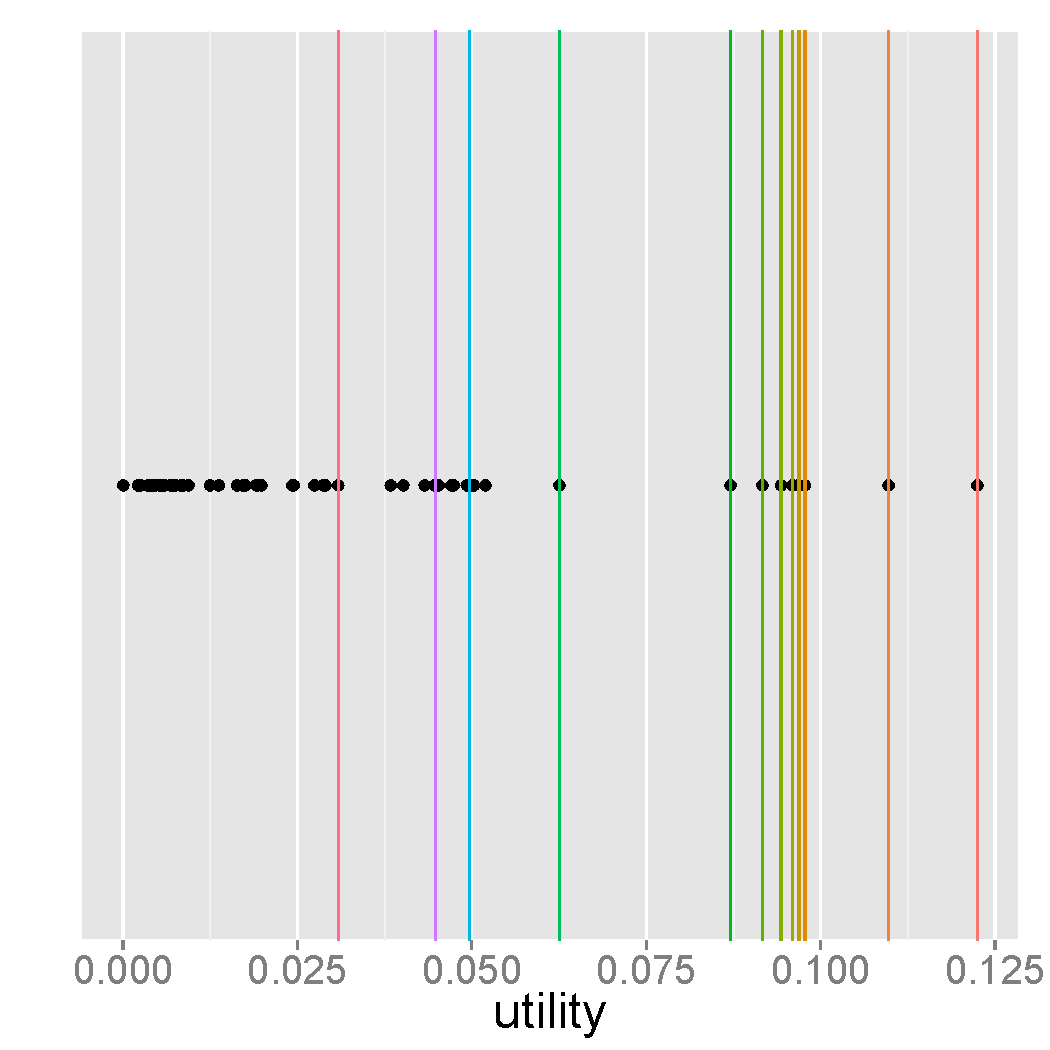
\includegraphics[trim = 0mm 50mm 0mm 50mm, clip, width=8cm]
		{Images/bank_utility_distribution.pdf}}
		\caption{Bank dataset: utility distribution}
		\label{fig:bank_utility_distribution}
	\end{subfigure}
	
	\begin{subfigure}{1\linewidth}
		\centering
		{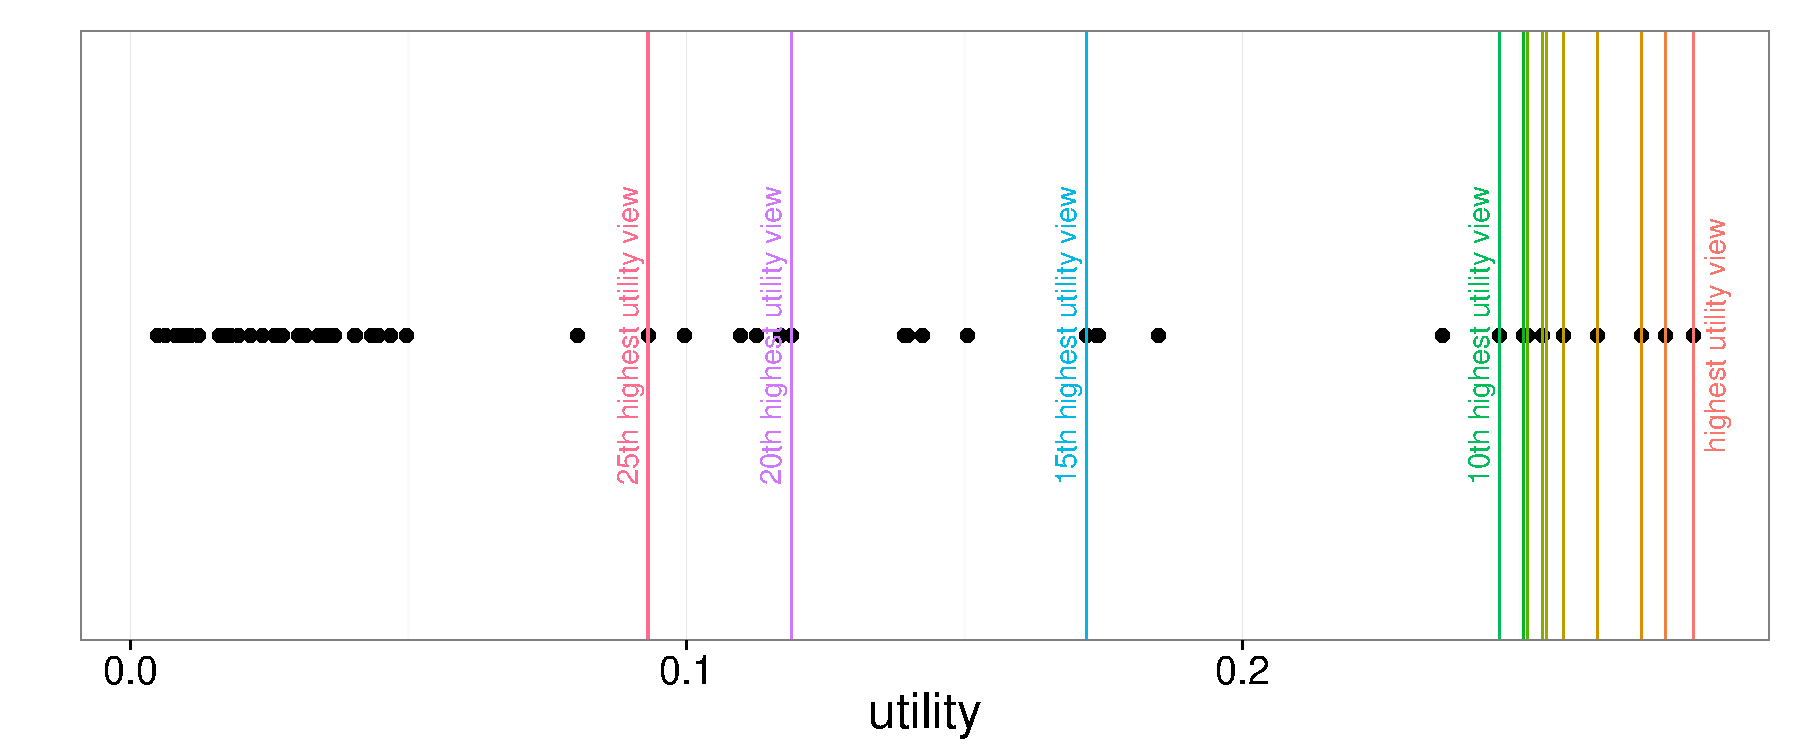
\includegraphics[trim = 0mm 50mm 0mm 50mm, clip, width=8cm]
		{Images/diabetes_utility_distribution.pdf}}
		\caption{Diabetes dataset: utility distribution}
		\label{fig:diabetes_utility_distribution}
	\end{subfigure}
\label{fig:utility_distribution}
\caption{Distribution of Utilities}
\end{figure}


\noindent {\it Accuracy and Utility Distance}:
Let us examine the banking dataset first.
The distribution of utilities for all views of the banking dataset is
shown in Figure \ref{fig:bank_utility_distribution}. 
In this chart, vertical lines denote the cutoffs for utilities for top-$k$ views
where $k$=\{1\ldots10,15,20,25\}.
The highest utility for this dataset corresponds to the {\it right-most} line
in this chart while the 25-th highest utility corresponds to the {\it left-most}
line.
We also observe other trends in this distribution of utilities: we see that the
highest and second highest utility are spread well apart from the rest of the
utilities.
We also observe that the top 3rd--9th utilities are rather similar. 
The 10th highest utility is separated from neighboring utilities by a large
value and then the remaining utilities are again close together.
This distribution of utilities directly impacts the performance of our pruning
techniques since utilities that are close together have very similar running
estimates of utility too and hence are difficult to lease apart and prune.
Utilities that are spread apart, in contrast, have estimates that are also
spread apart and we can prune views with high confidence.

We see that the impact of this utility distribution in the accuracy chart in
Figure \ref{fig:bank_accuracy}.
We find that the average accuracy of all three heuristics is pretty good for
$k$=1 and 2 (recall that these are spread apart from the other utilities).
However, between $k$=3\ldots9, the accuracy suffers (consequence of similar
utility values).
After $k$=10, the performance of all our heuristics improves once again.

Now, let us examine how ``bad'' our errors are in finding the top-$k$ views.
We do so by looking at the utility distance (i.e. the distance between
the average utility of the true top-$k$ views and the average utility of the
top-$k$ views picked by our heuristics).
Utility distance gives us an easy way to measure how far we are from the true
top-$k$ views.
Figure \ref{fig:bank_utility_dist} shows the utility distance for
all of our heuristics for the bank dataset.
The NO\_PRU technique necessarily has 0 utility distance since it performs no
pruning.
We notice, however, that all of our heuristics have 0 or almost 0 utility
distance (~0.003 on average).
This is there is effectively no difference in the utilities of the top $k$ views
we select vs. the true top-$k$ views.
So even when top-$k$ heuristic picks a few incorrect views, the selected views
have utility very close to the real top-$k$ views, i.e., are views are
approximate but of high quality.
% This implies that even if our top-$k$ views are
% approximate, they are of high quality.
% Another way to analyze mistakes in the top-$k$ views is by examining if the an
% incorrectly returned view for the top-$k$ views also appears in the top-$2k$,
% top-$3k$ or top-$4k$.
% Figure \ref{} shows the results for the banking dataset.
% We see that XXX,

\begin{figure*}[t]
	\centering
	\begin{subfigure}{0.33\linewidth}
		\centering
		{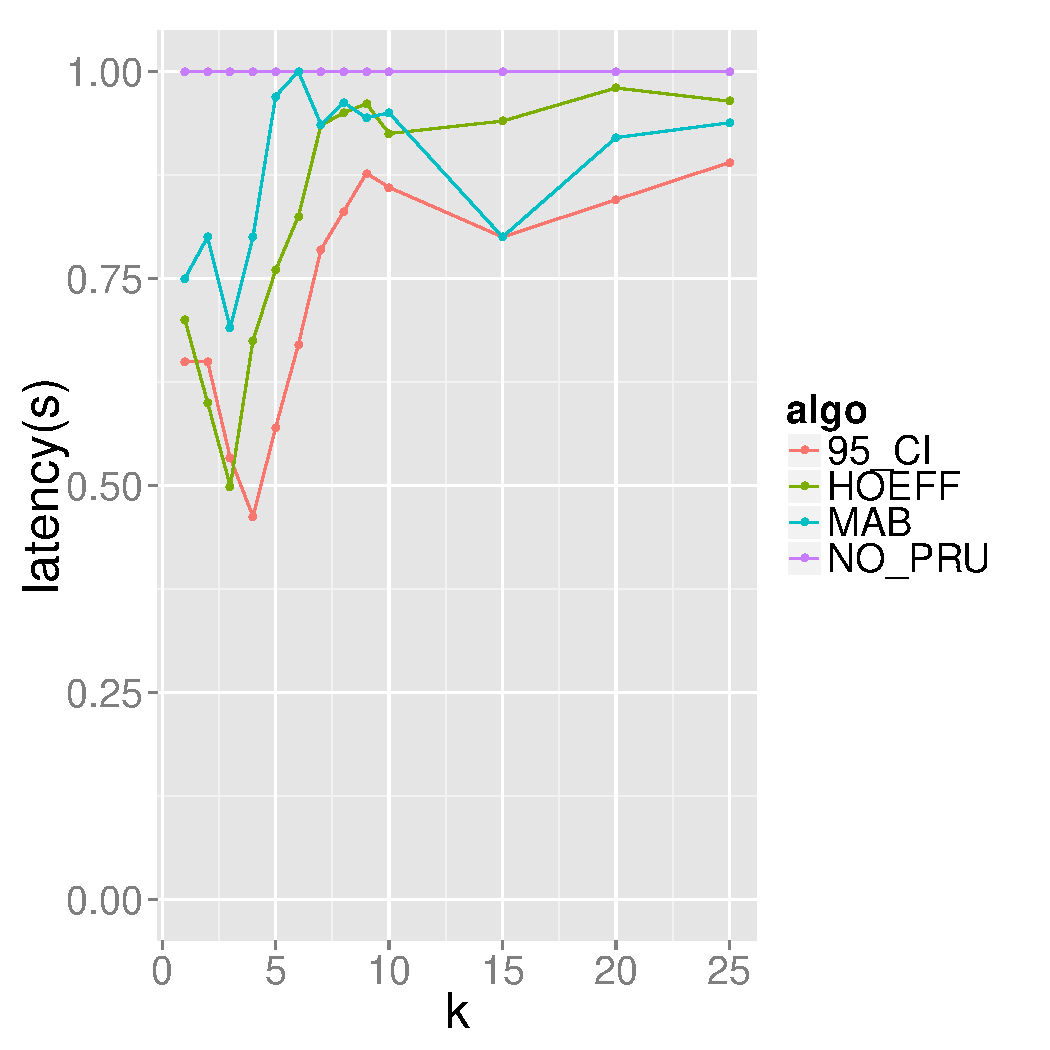
\includegraphics[width=6cm] {Images/bank_in_memory_accuracy.pdf}}
		\caption{Accuracy}
		\label{fig:bank_accuracy}
	\end{subfigure}
	\begin{subfigure}{0.33\linewidth}
		\centering
		{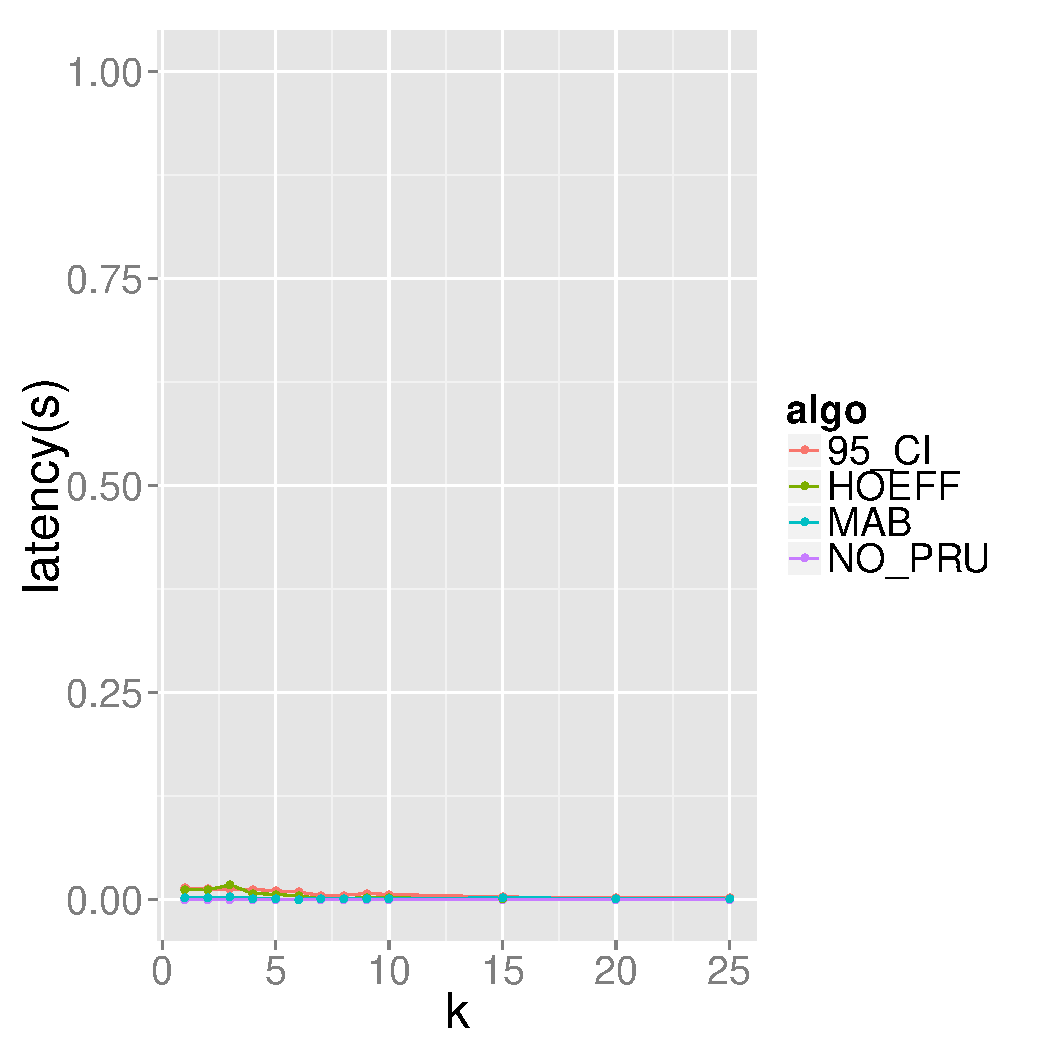
\includegraphics[width=6cm] {Images/bank_in_memory_utility_dist.pdf}}
		\caption{Utility Distance}
		\label{fig:bank_utility_dist}
	\end{subfigure}
	\begin{subfigure}{0.33\linewidth}
		\centering
		{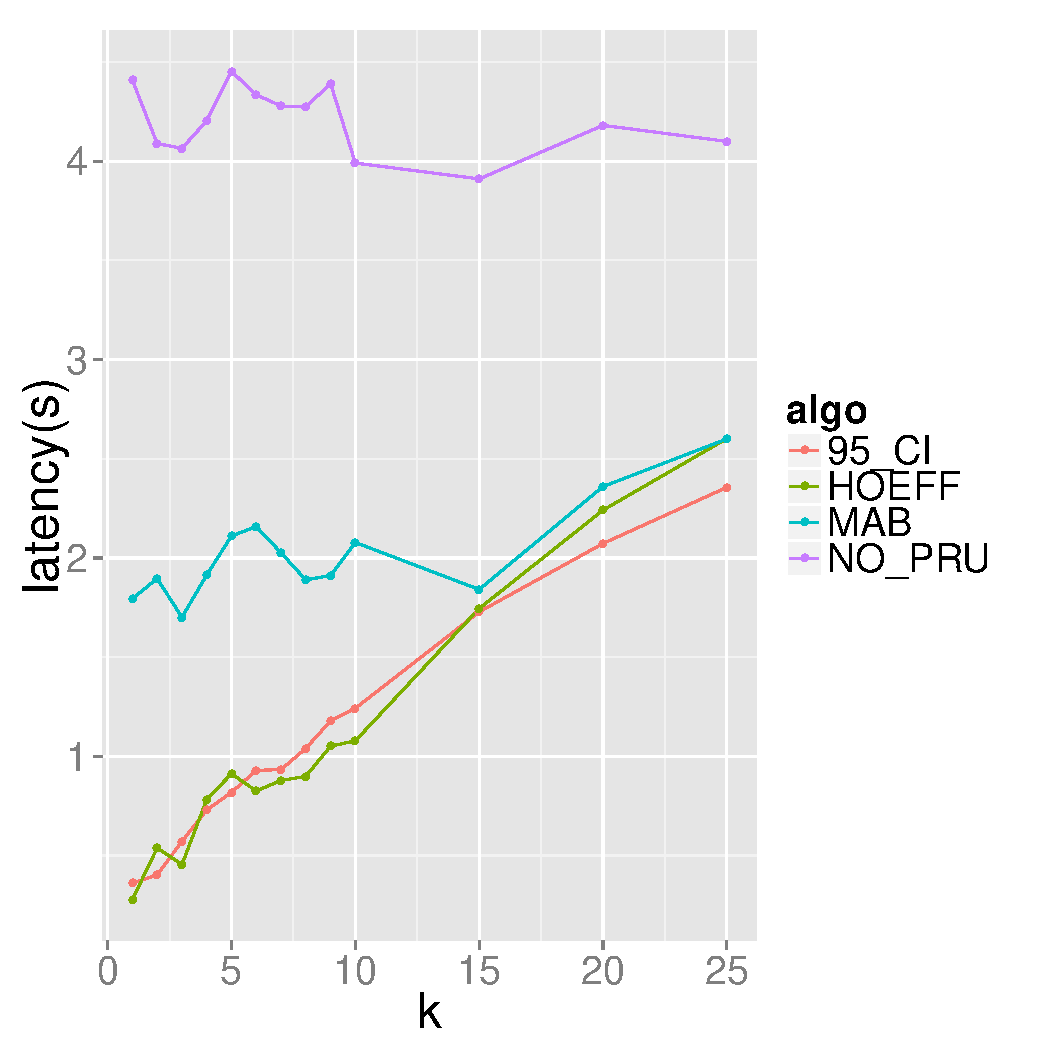
\includegraphics[width=6cm] {Images/bank_in_memory_latency.pdf}}
		\caption{Latency}
		\label{fig:bank_latency}
	\end{subfigure}
	\caption{Performance of heuristics for Bank dataset}
	\label{fig:bank_perf}
\end{figure*}

\begin{figure*}[t]
	\centering
	\begin{subfigure}{0.33\linewidth}
		\centering
		{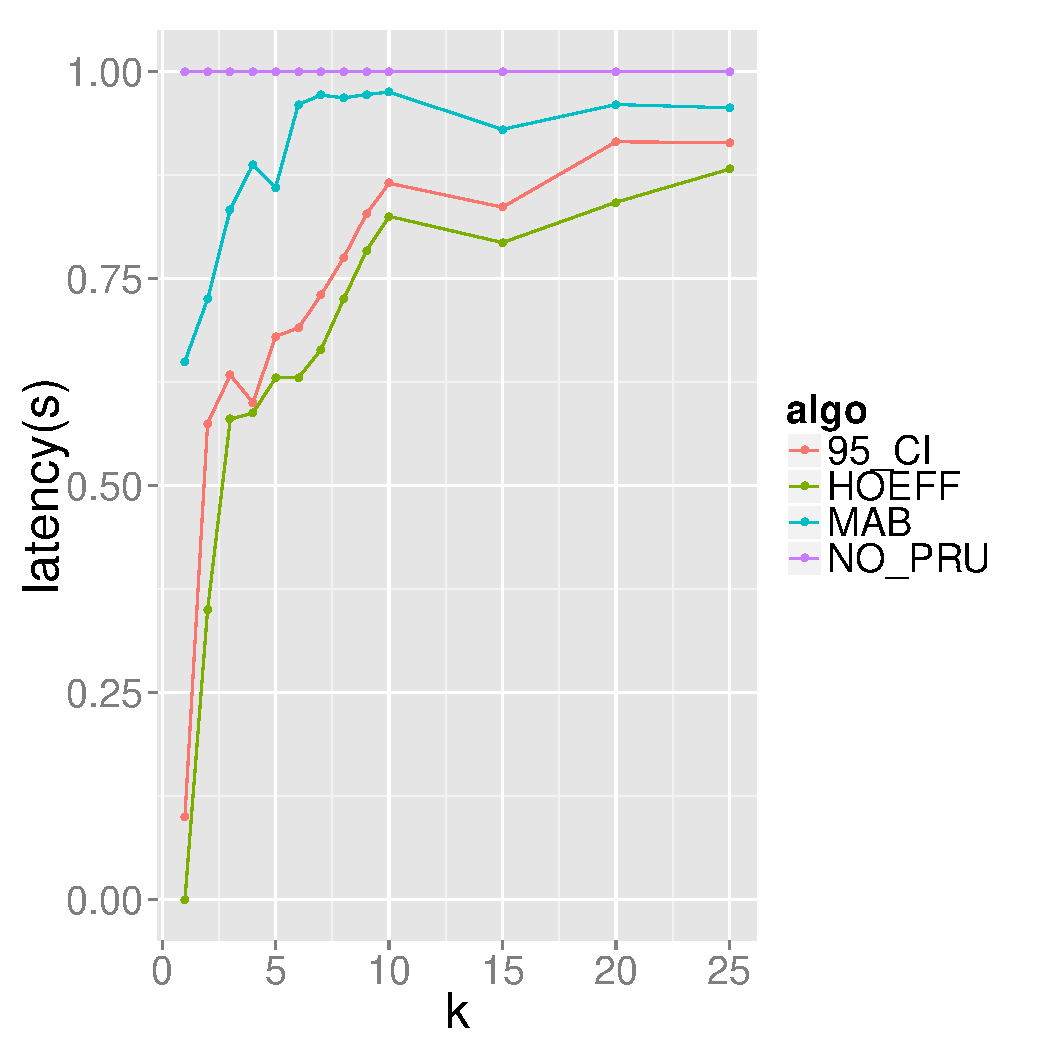
\includegraphics[width=6cm] {Images/dia_in_memory_accuracy.pdf}}
		\caption{Accuracy}
		\label{fig:dia_accuracy}
	\end{subfigure}
	\begin{subfigure}{0.33\linewidth}
		\centering
		{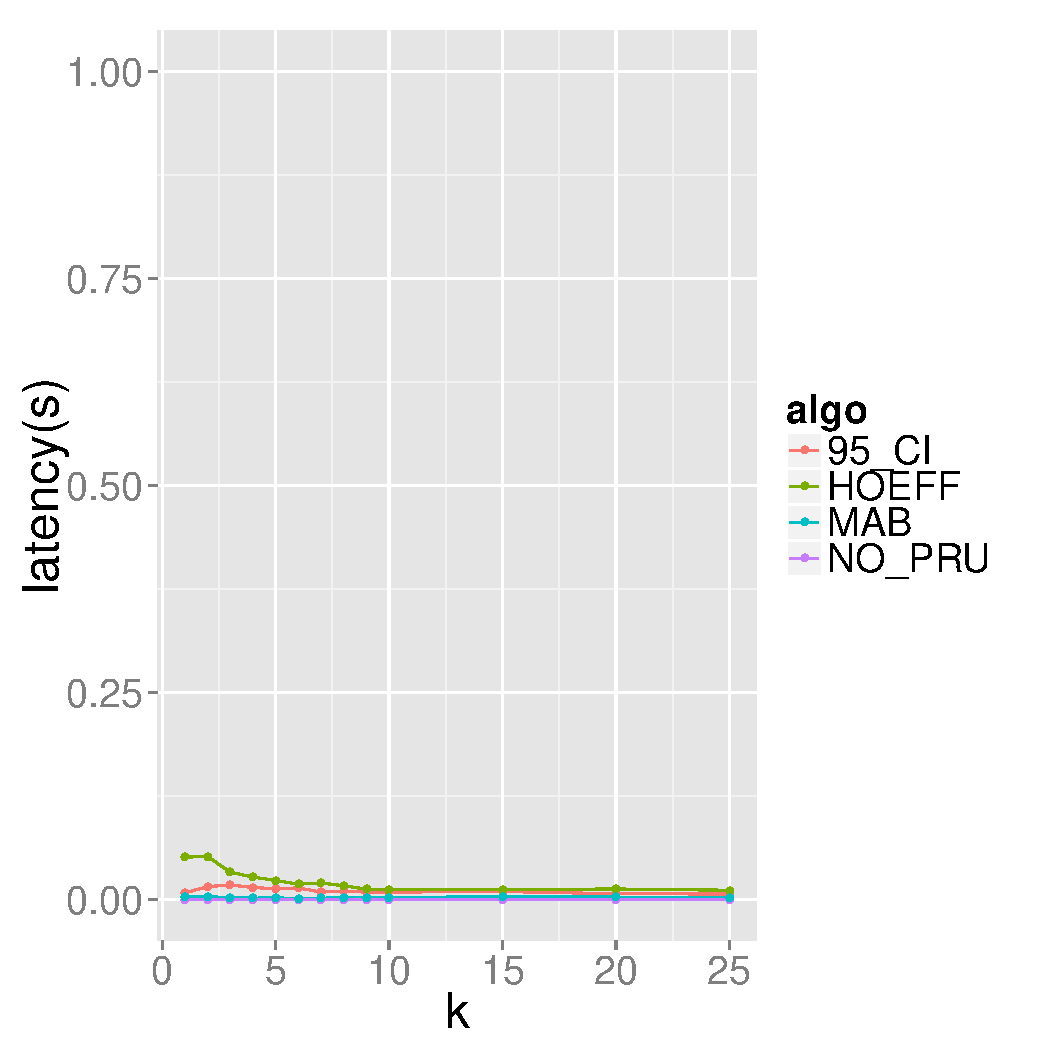
\includegraphics[width=6cm] {Images/dia_in_memory_utility_dist.pdf}}
		\caption{Utility Distance}
		\label{fig:dia_utility_dist}
	\end{subfigure}
	\begin{subfigure}{0.33\linewidth}
		\centering
		{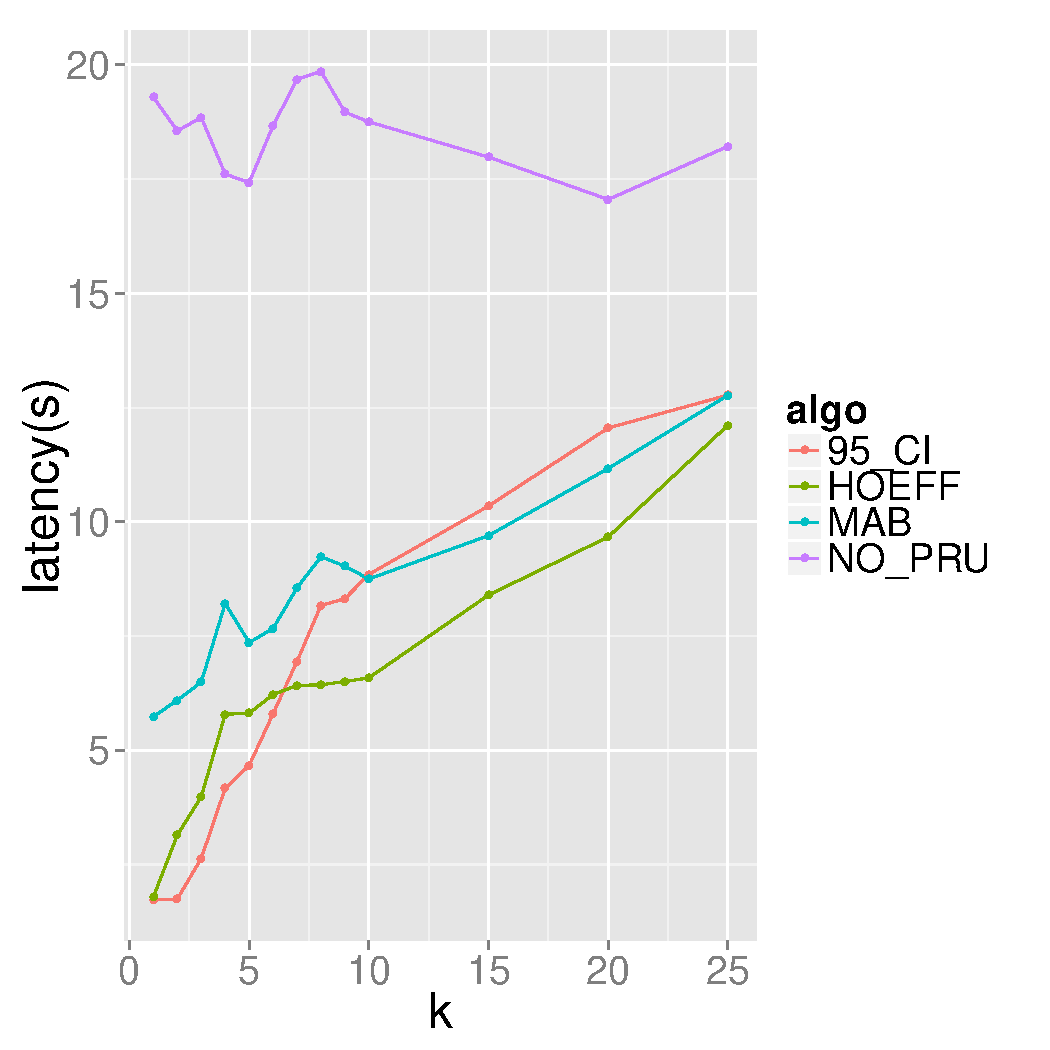
\includegraphics[width=6cm] {Images/dia_in_memory_latency.pdf}}
		\caption{Latency}
		\label{fig:diabetes_latency}
	\end{subfigure}
	\caption{Performance of heuristics for Diabetes dataset}
	\label{fig:diabetes_perf}
\end{figure*}

% \begin{figure}[h]
% \centering
% \begin{subfigure}{0.49\linewidth}
% \centering
% {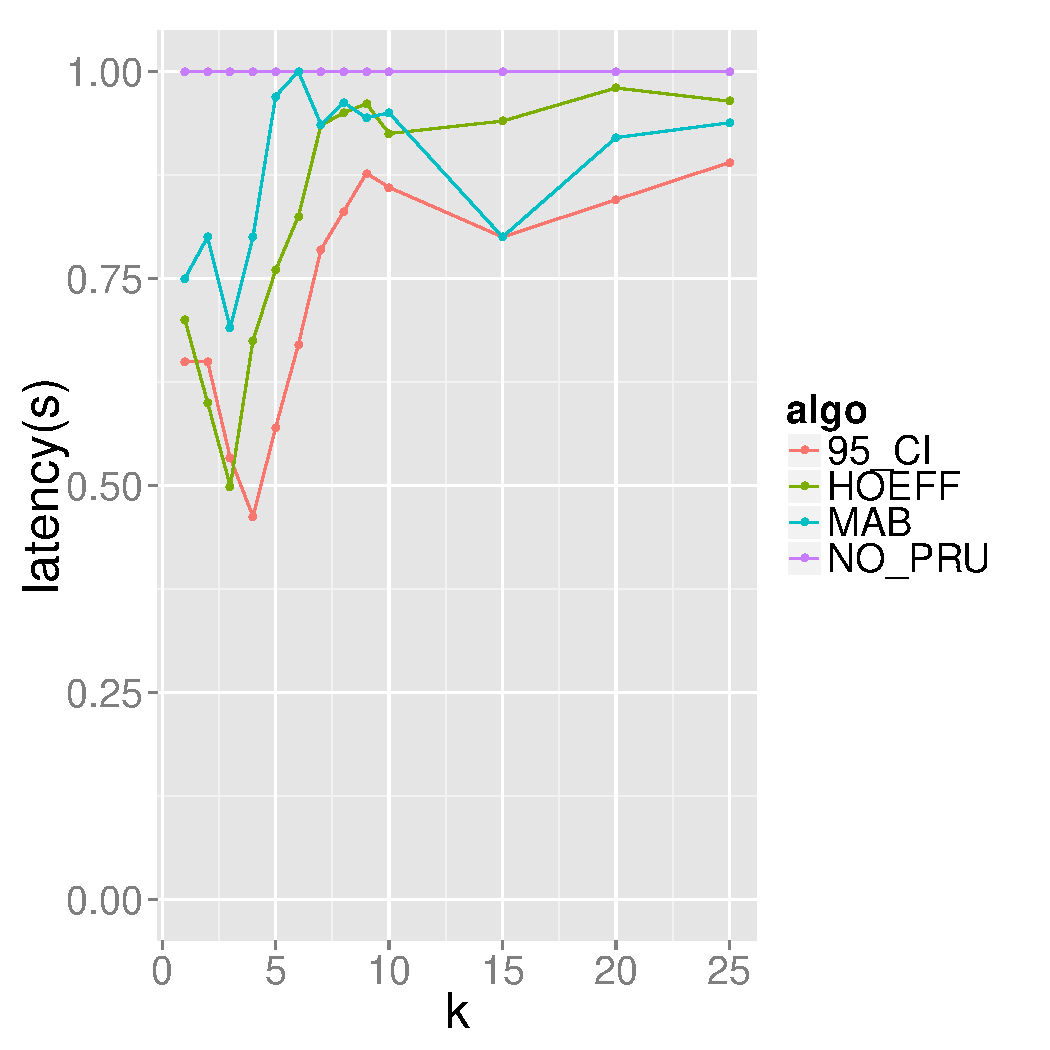
\includegraphics[width=4.2cm] {Images/bank_in_memory_accuracy.pdf}}
% \caption{Accuracy of heuristic for bank dataset}
% \label{fig:bank_accuracy}
% \end{subfigure}
% \begin{subfigure}{0.49\linewidth}
% \centering
% {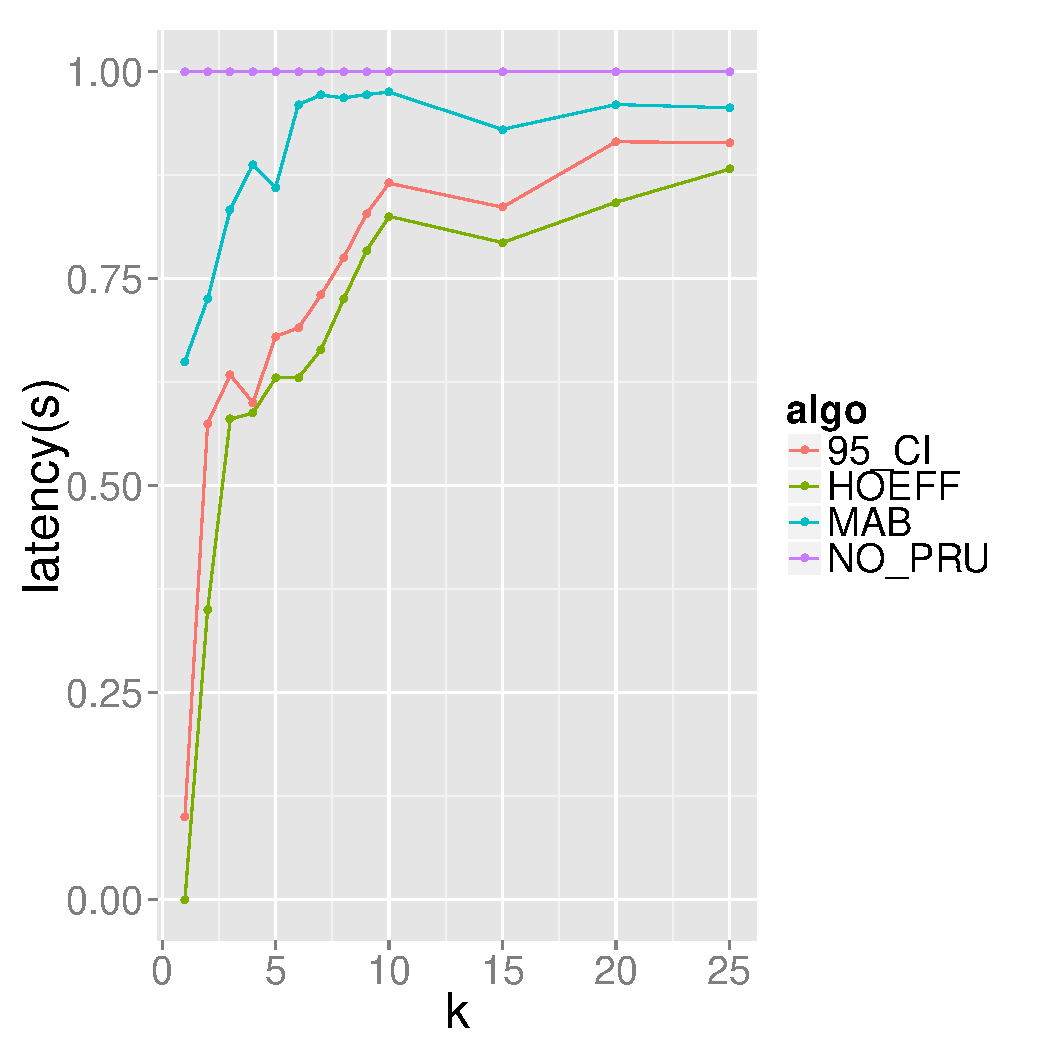
\includegraphics[width=4.2cm] {Images/dia_in_memory_accuracy.pdf}}
% \caption{Accuracy of heuristics for diabetes dataset}
% \label{fig:dia_accuracy}
% \end{subfigure}
% \label{fig:accuracy}
% \caption{Accuracy of Heuristics}
% \end{figure}


% \begin{figure}[h]
% \centering
% \begin{subfigure}{0.49\linewidth}
% \centering
% {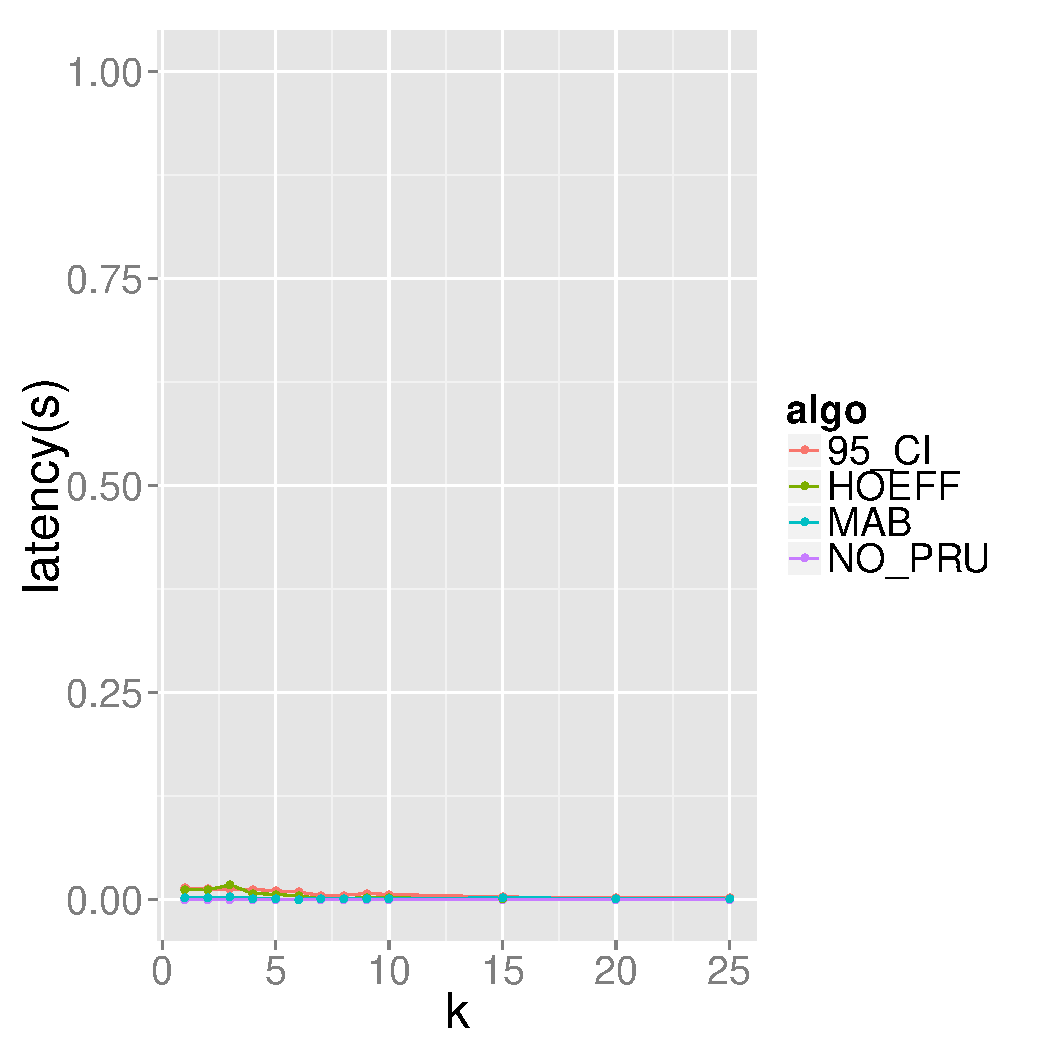
\includegraphics[width=4.2cm] {Images/bank_in_memory_utility_dist.pdf}}
% \caption{Utility Distance of heuristic for bank dataset}
% \label{fig:bank_utility_dist}
% \end{subfigure}
% \begin{subfigure}{0.49\linewidth}
% \centering
% {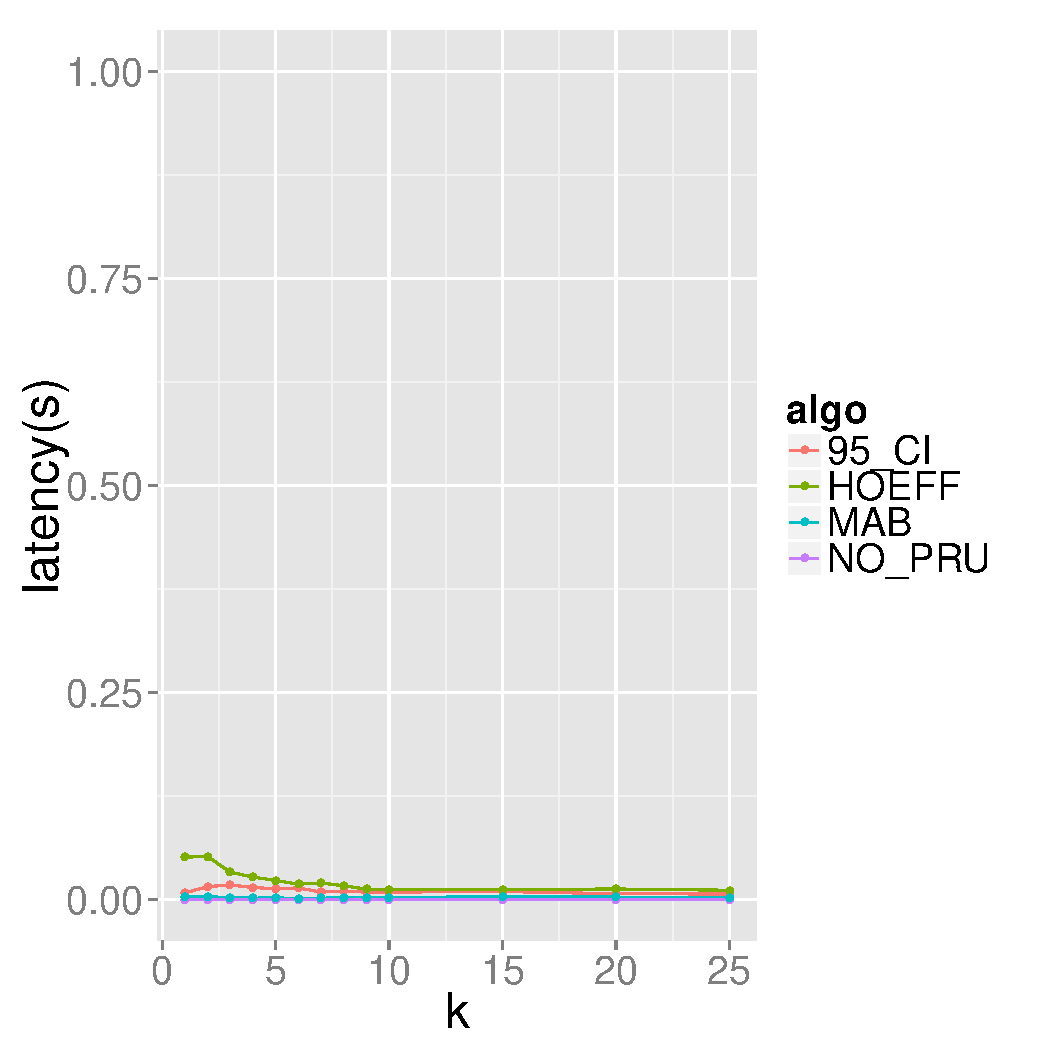
\includegraphics[width=4.2cm] {Images/dia_in_memory_utility_dist.pdf}}
% \caption{Utility Distance of heuristics for diabetes dataset}
% \label{fig:dia_utility_dist}
% \end{subfigure}
% \label{fig:accuracy}
% \caption{Utility Distance for Heuristics}
% \end{figure}

% \begin{figure}[h]
% \centering
% {\includegraphics[trim = 0mm 50mm 0mm 50mm, clip, width=6cm]
% {Images/bank_utility_distribution.pdf}}
% \caption{Bank dataset: utility distribution}
% \label{fig:bank_utility_distribution}
% \end{figure}
% \begin{figure}[h]
% \centering
% {\includegraphics[trim = 0mm 50mm 0mm 50mm, clip, width=6cm]
% {Images/diabetes_utility_distribution.pdf}}
% \caption{Diabetes dataset: utility distribution}
% \label{fig:diabetes_utility_distribution}
% \end{figure}
 
Next, let us examine the results for the diabetes dataset.
The distribution of true utilities for all views in this dataset are shown in
Figure \ref{fig:diabetes_utility_distribution}.
Compared to the bank dataset, we see that utilities are very closely
clustered for top 1\ldots10 views.
Compared to that, the utilities around $k$=15, 20 and 25 are relatively widlely
spaced.
As a result, we expect lower pruning accuracy for $k<10$ but high accuracy for
large $k$'s.
We see similar behavior in Figure \ref{fig:dia_accuracy} where the accuracy of
pruning is quite low for small $k$s, increases until $k$=10 and then levels off.
A similar trend is seen in Figure \ref{fig:dia_utility_dist} showing that
utility distance is small for $k<10$ and then reduces to almost 0.

We also observe an important property of our heuristics: the accuracy of all
three of our heuristics, MAB, 95\_CI and HOEFF, is comparable; MAB appears to
perform better for small number of $k$s but all three produce similar results
for $k>10$. (NO\_PRU is guaranteed to have perfect accuracy).
This suggests that since all heuristics perform similarly on accuracy, we can
choose the heuristic with the minimum latency.\\

% 95\_CI does the best among all our heuristics for the whole range of $k$ values.
% MAB and HOEFF produce similar accuracy values with MAB being slightly better
% than HOEFF.
% There are a few reasons why 95\_CI performs better: the MAB heuristic is tied to
% either accepting or discarding a view at the end of each phase; therefore, even
% if MAB is not very confidence in the action of accepting or discarding, it must
% reduce one view in each phase. HOEFF on the other hand is less accurate because
% XXX.
% All our heuristics however seem to have low accuracy for $k<10$. 

\noindent {\it Latency}:
Next, let us look at how long it takes for each of our pruning strategies to
work.
Figures \ref{fig:bank_latency} and \ref{fig:diabetes_latency} show the latency
of our heuristics for the banking and diabetes dataset.
The two charts look quite similar.
First off, we observe that {\it the use of any of our heuristics reduces the
latency by about 50\%}.
For NO\_PRU and 95\_CI, for small $k$'s, we obtain almost a 90\% reduction in
latency. However, as we saw earlier, some of this reduction in latency is
obtained at the cost lower accuracy.
We observe that the latency of HOEFF and 95\_CI increases almost linearly
with $k$.
Roughly speaking, this trend arises because as $k$
increases, we throw out fewer views and therforeperform more
computation for each record.
This exact trend is not seen in MAB because MAB's pruning of views is agnostic
to the number of views that must be selected.

In general, we see that it is possible to reduce latency by 50\% just by using
any of our heuristics.
If we want to achieve further performance gains, we must be willing to
tradeoff some accuracy.
The next set of experiments vary the parameters for each heuristic to study
the accuracy vs. latency tradeoff.\\

% \begin{figure}[h]
% \centering
% \begin{subfigure}{0.49\linewidth}
% \centering
% {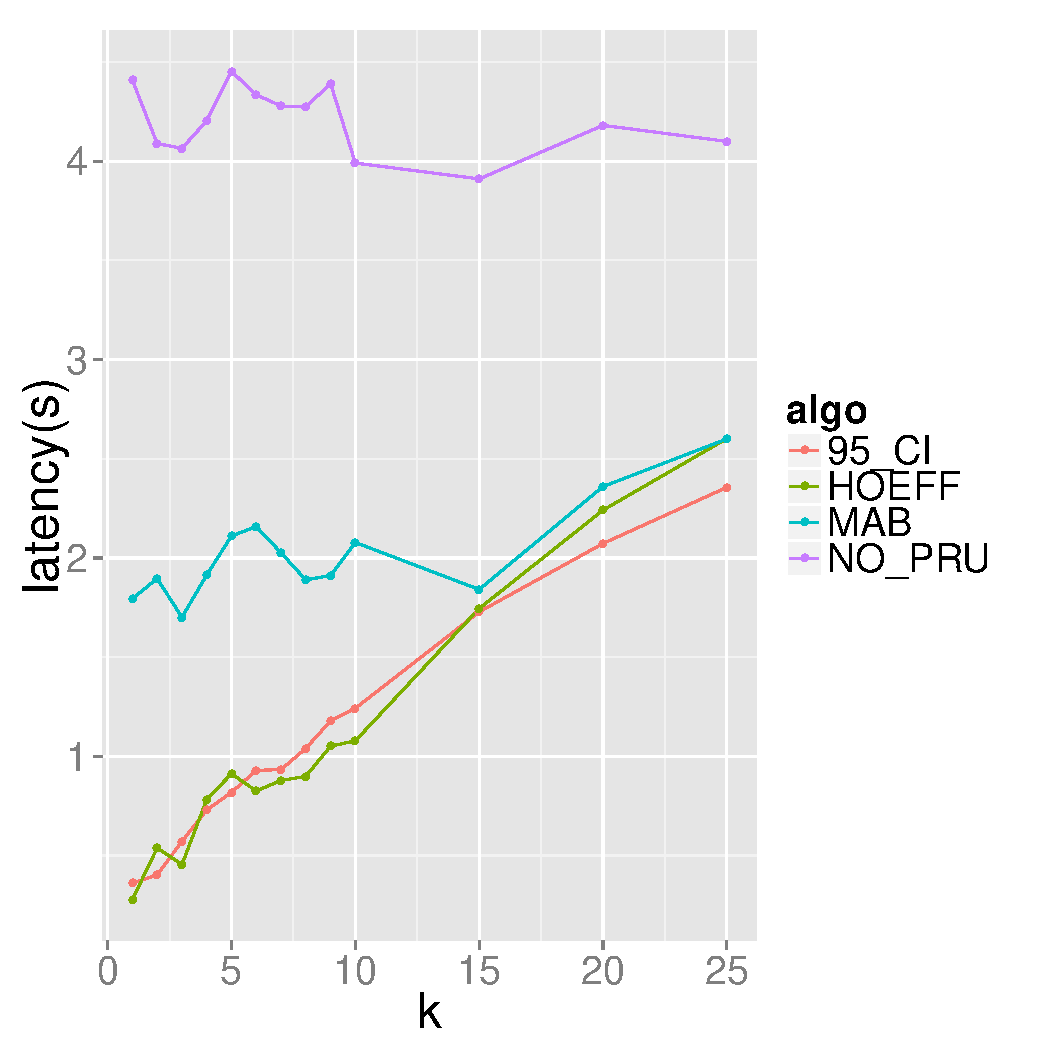
\includegraphics[width=4.2cm] {Images/bank_in_memory_latency.pdf}}
% \caption{Bank dataset: latency}
% \label{fig:bank_latency}
% \end{subfigure}
% \begin{subfigure}{0.49\linewidth}
% \centering
% {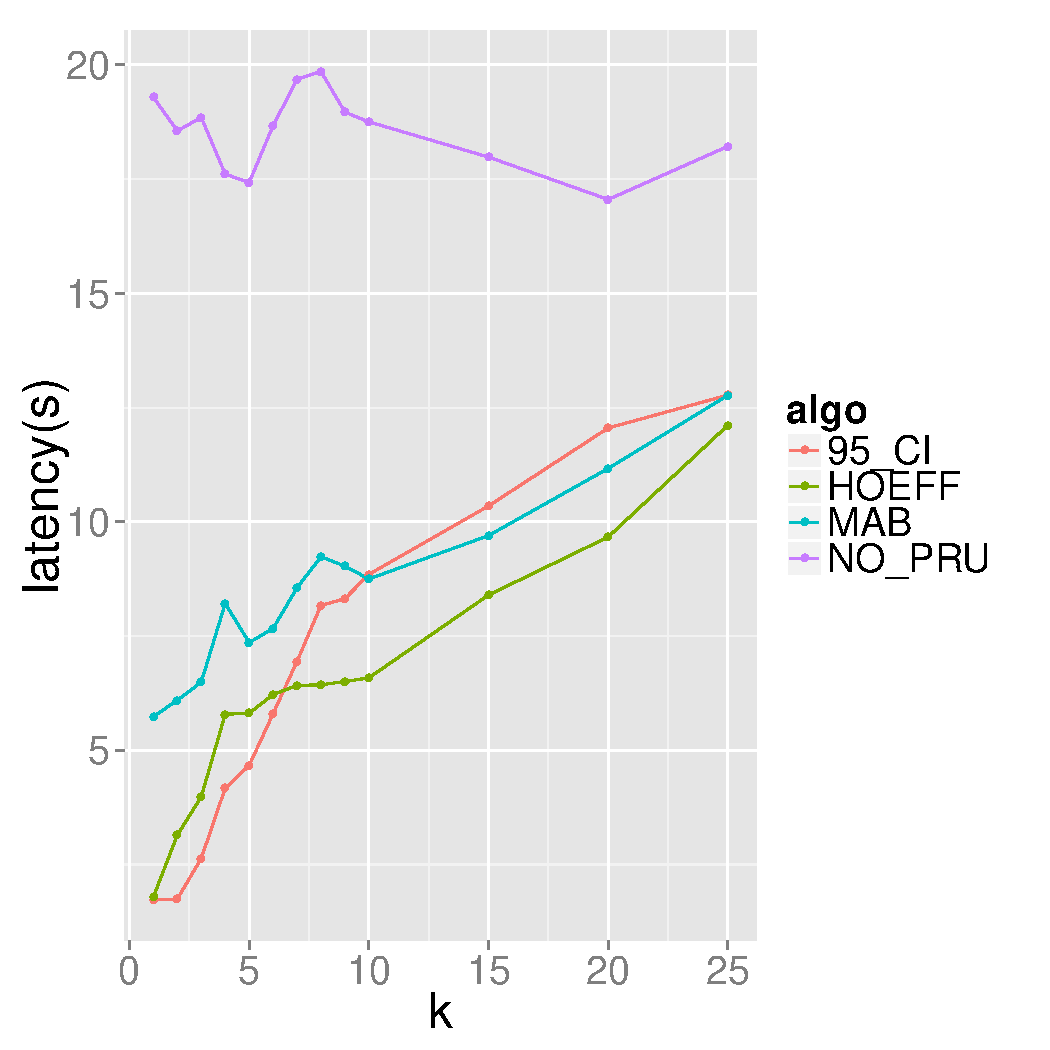
\includegraphics[width=4.2cm] {Images/dia_in_memory_latency.pdf}}
% \caption{Diabetes dataset: latency}
% \label{fig:diabetes_latency}
% \end{subfigure}
% \label{fig:accuracy}
% \caption{Latency for Heuristics}
% \end{figure}

\noindent {\it Accuracy vs. Latency}:
Our MAB and 95\_CI heuristics both have ``knobs'' we can use to study the
tradeoff between accuracy and latency.
In MAB, for example, we can tune the number of phases involved in
processing the entire file. 
Since MAB reduces the number of views by 1 after each phase, the number of
phases is proportional to the pruning power of our algorithm.
A large number of phases means that MAB will prune more views and will prune
them more often.
While this will lead to lower latency, it will also lead to lower accuracy.
Figure \ref{fig:latency_vs_accuracy_mab} shows how latency and accuracy both
reduce as we increase the number of phases in MAB.
Each point on the chart corresponds to a different setting for the number of
phases uses in that implementation of the MAB heuristic.
For 95\_CI, we can vary the $z$-score used
to determine the size of our confidence intervals.
That is, we can decide to take a 50\% confidence interval or a 80\% interval or
a 95\% interval.
If we take a smaller confidence interval, we will have higher pruning and
therefore lower latency.
However, a smaller confidence interval also leads to lower latency since we
prune views with lower confidence.
Figure \ref{fig:latency_vs_accuracy_ci} shows that as the $z$-score of the
confidence interval increases, the accuracy of our heuristics increases, but so
does its latency.
Every point corresponds to a different size of the confidence intervals.

\begin{figure}[h] 
\centering
\begin{subfigure}{0.49\linewidth}
\centering
{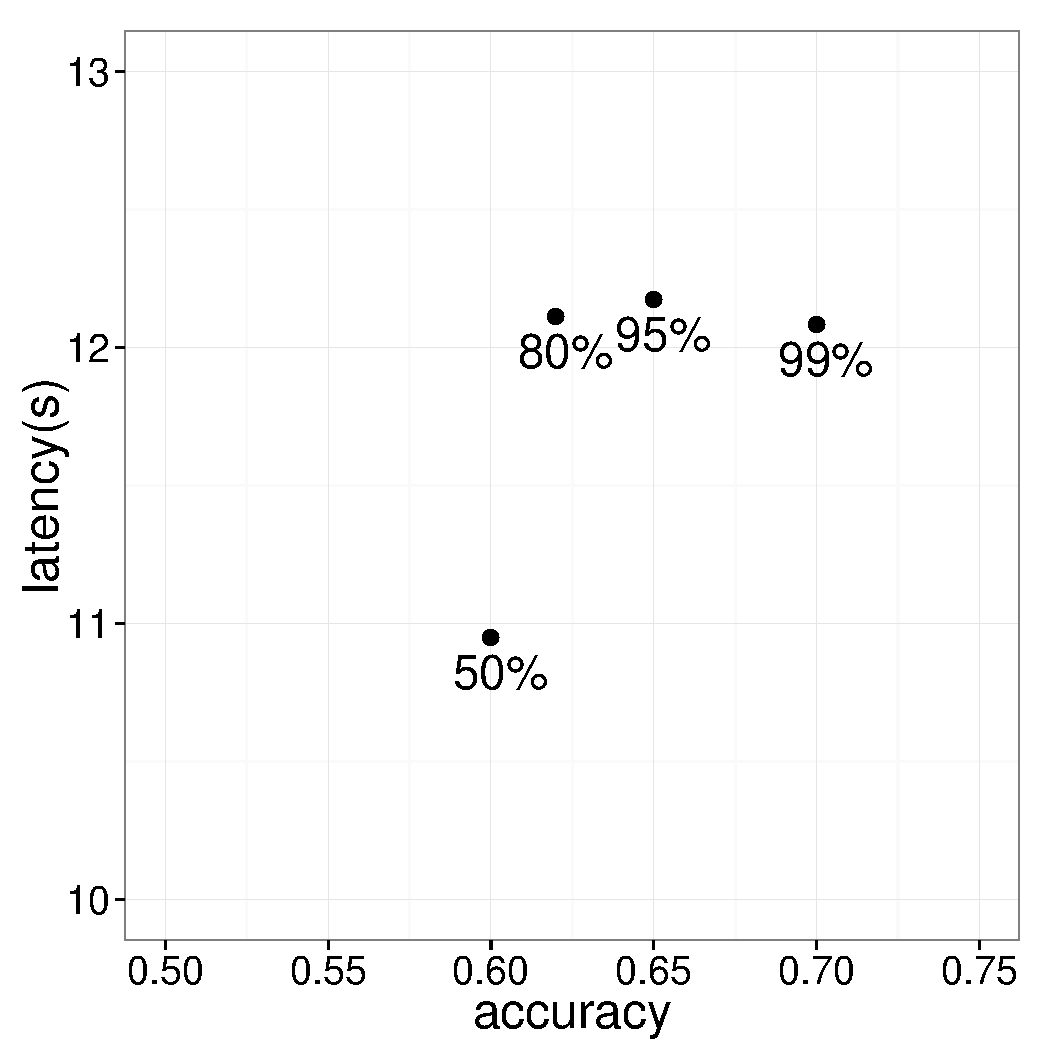
\includegraphics[width=4.2cm] {Images/latency_vs_accuracy_ci.pdf}}
\caption{Latency vs. Accuracy for CI-pruning}
\label{fig:latency_vs_accuracy_ci}
\end{subfigure}
\begin{subfigure}{0.49\linewidth}
\centering
{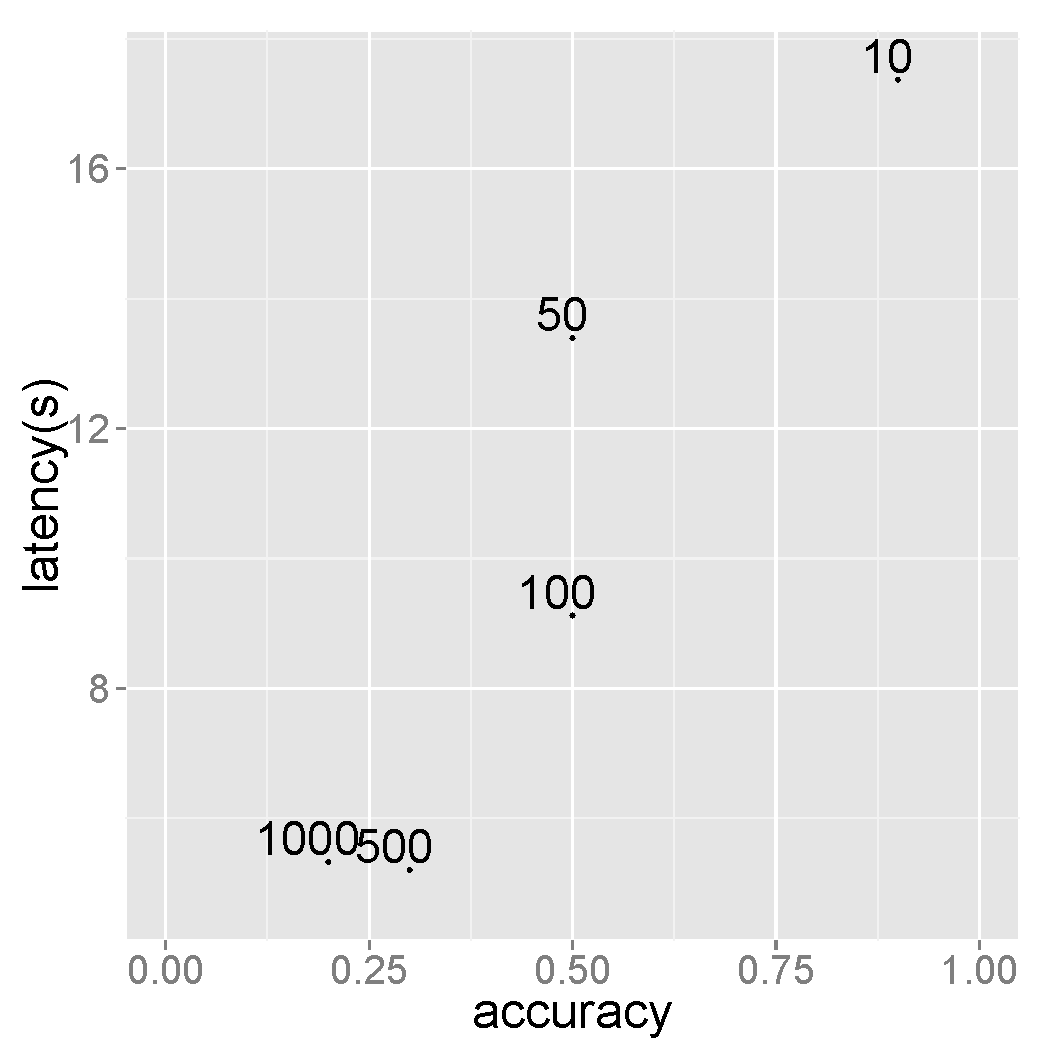
\includegraphics[width=4.2cm] {Images/latency_vs_accuracy_mab.pdf}}
\caption{Latency vs. Accuracy for MAB=pruning}
\label{fig:latency_vs_accuracy_mab}
\end{subfigure}
\label{fig:accuracy}
\caption{Latency vs. Accuracy for different heuristics}
\end{figure}

\subsection{Comparison of Execution Engines}

Now that we have examined the performance of both execution engines in detail,
we can make some comparisons across the two execution engines.
As mentioned before, we do not compare the latencies of both engines directly
since the implementations are not directly comparable.
However, we can summarize our findings as follows:
\squishlist
\item In general, column-stores provide better performance on the \VizRecDB\
workload although the workload involves reading every column in a table. This is
likely a consequence of the fact that our individual queries only read a few
columns at a time.
\item For row-stores, the combination of optimizations including combining
multiple aggregates, performing multiple group-bys and running queries in
parallel reduces latency by XXX\%, making \VizRecDB\ interaction possible in
near-interactive times.
\item For column-stores, we saw that the combination of multiple group-bys hurts
performance; however, combining aggregates and running queries in parallel
improves the already good performance of column stores getting response time
down to interactive times.
\item Our heuristics demonstrate that if we are willing to give up a small
amount of accuracy, we can reduce the \VizRecDB\ latency by a factor of 2. We
can also overcome the lower accuracy for small $k$'s by always querying for a
minumum number of views and only returning the top-$k$ views.
\item Finally, we see that if we are able to incorporate our heuristics into an
existing database system as discussed in Section \ref{}, we can expect to
obtain a similar 2X speedup. Along with the optimizations already developed for
the DBMS engine, these heuristics can enable \VizRecDB\ to respond within a
second.
\squishend







